% Options for packages loaded elsewhere
\PassOptionsToPackage{unicode}{hyperref}
\PassOptionsToPackage{hyphens}{url}
%
\documentclass[
]{book}
\usepackage{lmodern}
\usepackage{amssymb,amsmath}
\usepackage{ifxetex,ifluatex}
\ifnum 0\ifxetex 1\fi\ifluatex 1\fi=0 % if pdftex
  \usepackage[T1]{fontenc}
  \usepackage[utf8]{inputenc}
  \usepackage{textcomp} % provide euro and other symbols
\else % if luatex or xetex
  \usepackage{unicode-math}
  \defaultfontfeatures{Scale=MatchLowercase}
  \defaultfontfeatures[\rmfamily]{Ligatures=TeX,Scale=1}
\fi
% Use upquote if available, for straight quotes in verbatim environments
\IfFileExists{upquote.sty}{\usepackage{upquote}}{}
\IfFileExists{microtype.sty}{% use microtype if available
  \usepackage[]{microtype}
  \UseMicrotypeSet[protrusion]{basicmath} % disable protrusion for tt fonts
}{}
\makeatletter
\@ifundefined{KOMAClassName}{% if non-KOMA class
  \IfFileExists{parskip.sty}{%
    \usepackage{parskip}
  }{% else
    \setlength{\parindent}{0pt}
    \setlength{\parskip}{6pt plus 2pt minus 1pt}}
}{% if KOMA class
  \KOMAoptions{parskip=half}}
\makeatother
\usepackage{xcolor}
\IfFileExists{xurl.sty}{\usepackage{xurl}}{} % add URL line breaks if available
\IfFileExists{bookmark.sty}{\usepackage{bookmark}}{\usepackage{hyperref}}
\hypersetup{
  pdftitle={Introduzione a R},
  pdfauthor={Psicostat},
  hidelinks,
  pdfcreator={LaTeX via pandoc}}
\urlstyle{same} % disable monospaced font for URLs
\usepackage{longtable,booktabs}
% Correct order of tables after \paragraph or \subparagraph
\usepackage{etoolbox}
\makeatletter
\patchcmd\longtable{\par}{\if@noskipsec\mbox{}\fi\par}{}{}
\makeatother
% Allow footnotes in longtable head/foot
\IfFileExists{footnotehyper.sty}{\usepackage{footnotehyper}}{\usepackage{footnote}}
\makesavenoteenv{longtable}
\usepackage{graphicx,grffile}
\makeatletter
\def\maxwidth{\ifdim\Gin@nat@width>\linewidth\linewidth\else\Gin@nat@width\fi}
\def\maxheight{\ifdim\Gin@nat@height>\textheight\textheight\else\Gin@nat@height\fi}
\makeatother
% Scale images if necessary, so that they will not overflow the page
% margins by default, and it is still possible to overwrite the defaults
% using explicit options in \includegraphics[width, height, ...]{}
\setkeys{Gin}{width=\maxwidth,height=\maxheight,keepaspectratio}
% Set default figure placement to htbp
\makeatletter
\def\fps@figure{htbp}
\makeatother
\setlength{\emergencystretch}{3em} % prevent overfull lines
\providecommand{\tightlist}{%
  \setlength{\itemsep}{0pt}\setlength{\parskip}{0pt}}
\setcounter{secnumdepth}{5}
\usepackage{booktabs}
\usepackage{amsthm}
\makeatletter
\def\thm@space@setup{%
  \thm@preskip=8pt plus 2pt minus 4pt
  \thm@postskip=\thm@preskip
}
\makeatother


%----    define infoboxes    ----%
\usepackage{tcolorbox}
\usepackage{xcolor}

% colors
\definecolor{background}{HTML}{fcfcfc}
\definecolor{tip-text}{HTML}{e7b002}
\definecolor{tip-line}{HTML}{fdce38}
\definecolor{warning-text}{HTML}{b06336}
\definecolor{warning-line}{HTML}{c97d50}
\definecolor{deffun-text}{HTML}{0b797e}
\definecolor{deffun-line}{HTML}{6CC2C9}
\definecolor{design-text}{HTML}{7c972e}
\definecolor{design-line}{HTML}{a7c84a}
\definecolor{trick-text}{HTML}{8c3031}
\definecolor{trick-line}{HTML}{A3595A}

\newtcolorbox{mybox}[1][black]{
  colback=background,
  coltext=black,
  colframe=#1,
  boxsep=5pt,
  arc=4pt}

% tip
\newenvironment{tip}[1][Title]
  {
  \setlength{\fboxsep}{1em}
  \begin{mybox}[tip-line]
    \raisebox{-.2\height}{
\includegraphics[height=.6cm]{images/lightbulb.png}} \large \textcolor{tip-text}{Tip-Box: #1}\\
    }
    {
  \end{mybox}
  }

% warning
\newenvironment{warning}[1][Title]
  {
  \setlength{\fboxsep}{1em}
  \begin{mybox}[warning-line]
    \raisebox{-.2\height}{
\includegraphics[height=.6cm]{images/gotcha.png}} \large \textcolor{warning-text}{Warning-Box: #1}\\
    }
    {
  \end{mybox}
  }

% deffun
\newenvironment{deffun}[1][Title]
  {
  \setlength{\fboxsep}{1em}
  \begin{mybox}[deffun-line]
    \raisebox{-.2\height}{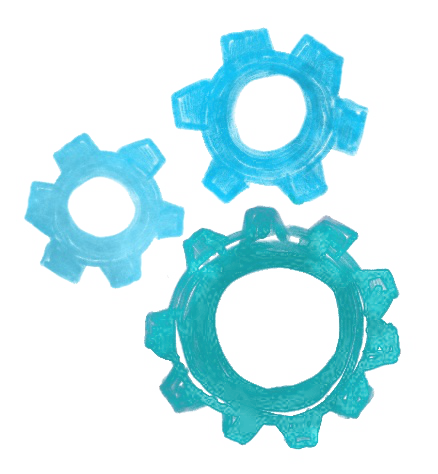
\includegraphics[height=.6cm]{images/gears.png}} \large \textcolor{deffun-text}{Definition-Box: #1}\\
    }
    {
  \end{mybox}
  }

% design
\newenvironment{design}[1][Title]
  {
  \setlength{\fboxsep}{1em}
  \begin{mybox}[design-line]
    \raisebox{-.2\height}{
\includegraphics[height=.6cm]{images/design.png}} \large \textcolor{design-text}{Approfondimento: #1}\\
    }
    {
  \end{mybox}
  }

% trick
\newenvironment{trick}[1][Title]
  {
  \setlength{\fboxsep}{1em}
  \begin{mybox}[trick-line]
    \raisebox{-.2\height}{
\includegraphics[height=.6cm]{images/hat.png}} \large \textcolor{trick-text}{Trick-Box: #1}\\
    }
    {
  \end{mybox}
  }
\usepackage{titlepic}
\titlepic{
\includegraphics[width=\textwidth]{images/logo_psicostat.pdf}}
\usepackage[]{natbib}
\bibliographystyle{plainnat}

\title{{Introduzione a R}}
\usepackage{etoolbox}
\makeatletter
\providecommand{\subtitle}[1]{% add subtitle to \maketitle
  \apptocmd{\@title}{\par {\large #1 \par}}{}{}
}
\makeatother
\subtitle{Corso per imparare le basi di \textbf{R}}
\author{\href{https://psicostat.dpss.psy.unipd.it/}{Psicostat}}
\date{11-03-2021}

\begin{document}
\maketitle

{
\setcounter{tocdepth}{1}
\tableofcontents
}
\hypertarget{presentazione}{%
\chapter*{Presentazione}\label{presentazione}}
\addcontentsline{toc}{chapter}{Presentazione}

In questo libro impareremo le basi di \emph{R}, uno dei migliori software per la visualizzazione e l'analisi statistica dei dati. Partiremo da zero intorducendo gli aspetti fondamentili di R e i concetti alla base di ogni linguaggio di programmazione che ti pemetteranno in seguito di approfondire e sviluppare le tue abilità in questo bellissimo mondo.

\hypertarget{perchuxe8-r}{%
\section*{Perchè R}\label{perchuxe8-r}}
\addcontentsline{toc}{section}{Perchè R}

Ci sono molte ragioni per cui scegliere R rispetto ad altri programmi usati per condurre le analisi statistiche. Innanzitutto è un linguaggio di programmazione (come ad esempio Python, Java, C++, o Julia) e non semplicemente un'interfaccia punta e clicca (come ad esempio SPSS o JASP). Questo comporta si maggiori difficoltà iniziali ma ti ricompenserà in futuro poichè avari imparato ad utilizza uno strumennto molto potente.

Inoltre, R è:

\begin{itemize}
\tightlist
\item
  nato per la statistica
\item
  open-source
\item
  ricco di pacchetti
\item
  supportato da una grande comunità
\item
  gratis
\end{itemize}

\hypertarget{struttura-del-libro}{%
\section*{Struttura del libro}\label{struttura-del-libro}}
\addcontentsline{toc}{section}{Struttura del libro}

Il libro è suddiviso in quattro sezioni principali:

\begin{itemize}
\tightlist
\item
  \textbf{Get started}. Una volta installato R ed RStudio, famiglierizzeremo con l'ambiente di lavoro introducendo alcuni aspetti generali e le funzioni principali. Verranno inoltre descritte alcune buone regole per iniziare una sessione di lavoro in R.
\item
  \textbf{Struttura dei dati}. Impareremo gli oggetti principali che R utilizza al suo interno. Variabili, vettori, matrici, dataframe e liste non avranno più segreti e capiremo come manipolarli e utlizzarli a seconda delle varie necessità.
\item
  \textbf{Algoritmi}. Non farti spaventare da questo nome. Ne avrai spesso sentito parlarne come qualcosa di molto complicato, ma in realtà gli algoritmi sono semplicemente una serie di istruzioni che il computer segue quando deve eseguire un determinato compito. In questa sezione vedremo i principali comandi di R usati per definire degli algoritmi. Questo è il vantaggio di conoscere un linguaggio di programmazione, ci permette di creare nuovi programmi che il computer eseguirà per noi.
\item
  \textbf{Case study}. Eseguiremo passo per passo un analisi che ci permetterà di imparare come importare i dati, codificare le variabili, manipolare e preprare i dati perle analisi, condurre delle analisi descrittive e creare dei grafici.
\end{itemize}

Alla fine di questo libro probabilmente non sarete assunti da Google, ma speriamo almeno che R non vi faccia più così paura e che magari a qualcuno sia nato l'interesse di approfondire questo fantastico mondo fatto di linee di codice.

\hypertarget{risorse-utili}{%
\section*{Risorse Utili}\label{risorse-utili}}
\addcontentsline{toc}{section}{Risorse Utili}

Segnaliamo qui per il lettore interessato del materiale online (in inglese) per approfondire le conoscenze sull'uso di R.

Materiale introduttivo:

\begin{itemize}
\tightlist
\item
  \emph{R for Psychological Science} di Danielle Navarro \url{https://psyr.djnavarro.net/index.html}
\item
  \emph{Hands-On Programming with R} di Garrett Grolemund \url{https://rstudio-education.github.io/hopr/}
\end{itemize}

Materiale intermedio:

\begin{itemize}
\tightlist
\item
  \emph{R for Data Science} di Hadley Wickham e Garrett Grolemund \url{https://r4ds.had.co.nz/}
\end{itemize}

Materiale avanzato:

\begin{itemize}
\tightlist
\item
  \emph{R Packages} di Hadley Wickham e Jennifer Bryan \url{https://r-pkgs.org/}
\item
  \emph{Advanced R} di Hadley Wickham \url{https://adv-r.hadley.nz/}
\end{itemize}

\hypertarget{psicostat}{%
\section*{Psicostat}\label{psicostat}}
\addcontentsline{toc}{section}{Psicostat}

Questo libro è stato prodotto da \textbf{Psicostat}, un gruppo di ricerca interdisciplinare dell'universita di Padova che unisce la passione per la statistica e la psicologia. Se vuoi conoscere di più riguardo le nostre attività visita il nosto sito \url{https://psicostat.dpss.psy.unipd.it/} o aggiungiti alla nostra mailing list \url{https://lists.dpss.psy.unipd.it/postorius/lists/psicostat.lists.dpss.psy.unipd.it/}.

\hypertarget{collaborazione}{%
\section*{Collaborazione}\label{collaborazione}}
\addcontentsline{toc}{section}{Collaborazione}

Se vuoi collaborare alla revione e scrittura di questo libro (ovviamente è tutto in R) visita la nostra repository di Github \url{https://github.com/psicostat/Introduction2R}.

\hypertarget{riconoscimenti}{%
\section*{Riconoscimenti}\label{riconoscimenti}}
\addcontentsline{toc}{section}{Riconoscimenti}

Il template di questo libro è basato su \href{https://github.com/rstudio/bookdown-demo}{Rstudio Bookdown-demo} rilasciato con licenza \href{https://creativecommons.org/publicdomain/zero/1.0/}{CC0-1.0} e \href{https://rstudio4edu.github.io/rstudio4edu-book/}{rstudio4edu-book} rilasciato con licenza \href{https://creativecommons.org/licenses/by/2.0/}{CC BY}. Nota che le illustrazioni utilizzate nelle vignette appartengono sempre a \href{https://rstudio4edu.github.io/rstudio4edu-book/}{rstudio4edu-book} e sono rilasciate con licenza \href{https://creativecommons.org/licenses/by-nc/2.0/}{CC BY-NC}.

\hypertarget{licenza}{%
\section*{Licenza}\label{licenza}}
\addcontentsline{toc}{section}{Licenza}

Questo libro è rilasciato sotto la Creative Commons Attribution-ShareAlike 4.0 International Public License (\href{https://creativecommons.org/licenses/by-sa/4.0/legalcode}{CC BY-SA}).
Le illustrazioni utilizzate nelle vignette appartengono a \href{https://rstudio4edu.github.io/rstudio4edu-book/}{rstudio4edu-book} e sono rilasciate con licenza \href{https://creativecommons.org/licenses/by-nc/2.0/}{CC BY-NC}.

\hypertarget{part-get-started}{%
\part*{Get Started}\label{part-get-started}}
\addcontentsline{toc}{part}{Get Started}

\hypertarget{intorduzione}{%
\chapter*{Intorduzione}\label{intorduzione}}
\addcontentsline{toc}{chapter}{Intorduzione}

In questa sezione verranno presentate le istruzioni per installare R ed RStudio. In seguito, famiglierizzeremo con l'ambiente di lavoro introducendo alcuni aspetti generali e le funzioni principali. Verranno inoltre descritte alcune buone regole per iniziare una sessione di lavoro in R.

I capitoli sono così organizzati:

\begin{itemize}
\tightlist
\item
  \textbf{Capitolo \ref{install}: Installare R e RStudio}. Instruzioni passo a passo per installare R e RStudio
\item
  \textbf{Capitolo \ref{first-commands}: Primi Passi in R}. Introduzione all'interfaccia di RStudio, operatori matematici, operatori logici, creazione di variabili e utilizzo di funzioni.
\item
  \textbf{Capitolo \ref{working-session}: Sessione di Lavoro}. Utilizzo degli script e introduzione dei concetti di environment, working directory e pacchetti di R.
\end{itemize}

\hypertarget{install}{%
\chapter{Installare R e RStudio}\label{install}}

R ed R-studio sono due software distinti. R è un linguaggio di programmazione usato in particolare in ambiti quali la statistica. R-studio invece è un'interfaccia \emph{user-friendly} che permette di utilizzare R.
R può essere utilizzato autonomamente tuttavia è consigliato l'utilizzo attraverso R-studio. Entrambi vanno installati separatamente e la procedura varia a seconda del proprio sistema operativo (Windows, MacOS o Linux). Riportiamo le istruzioni solo per Windows e MacOS. Chi utilizza Linux sicuramente è autonomo nell'installazione di questi due semplici programmi.

\hypertarget{installare-r}{%
\section{Installare R}\label{installare-r}}

\begin{enumerate}
\def\labelenumi{\arabic{enumi}.}
\tightlist
\item
  Accedere al sito \url{https://www.r-project.org}
\item
  Selezionare la voce \textbf{CRAN} (Comprehensive R Archive Network) dal menù di sinistra sotto \textbf{Download}
\end{enumerate}

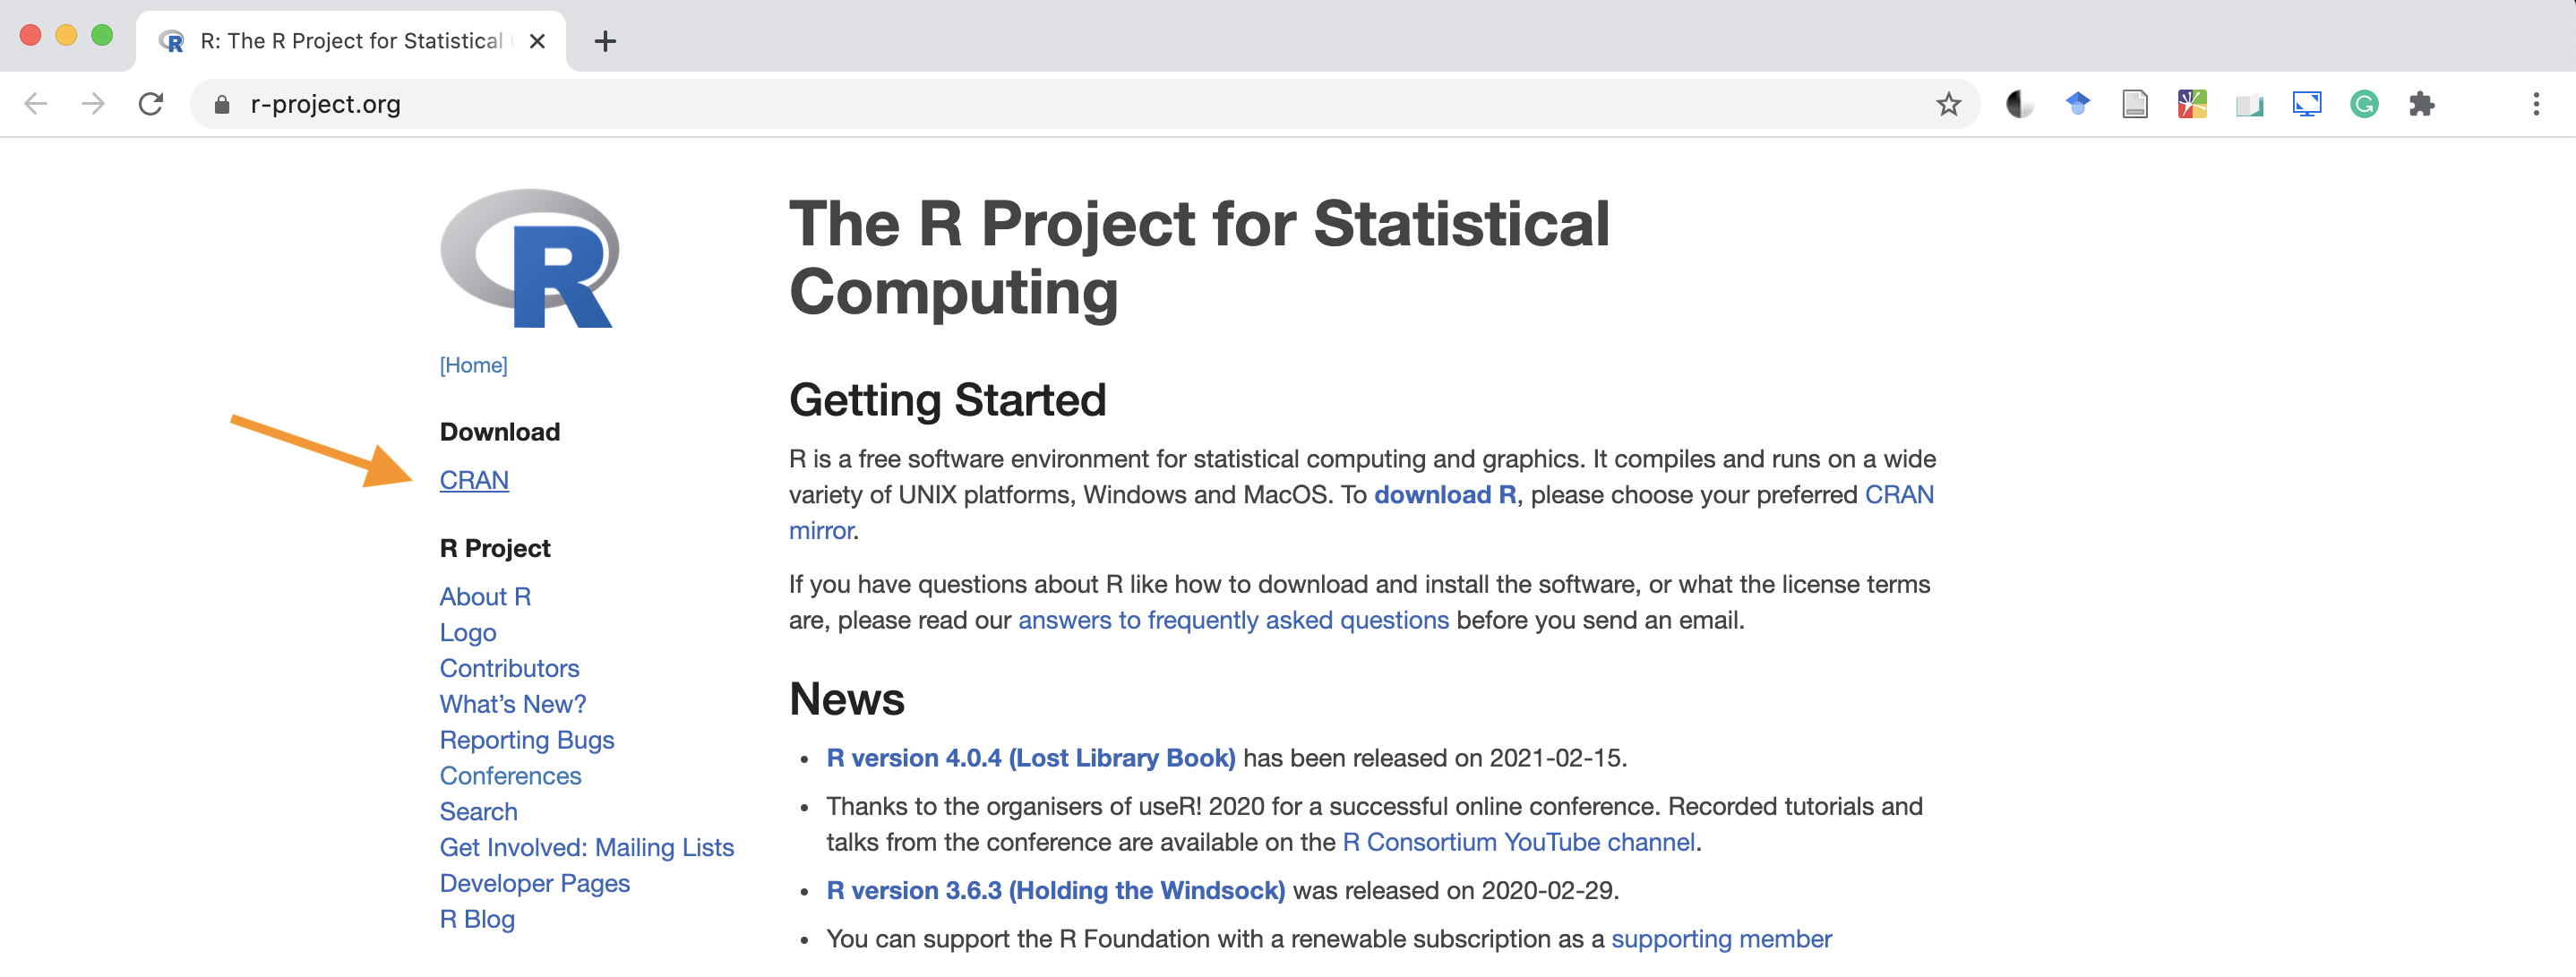
\includegraphics[width=0.95\textwidth,height=\textheight]{images/install_CRAN.png}

\begin{enumerate}
\def\labelenumi{\arabic{enumi}.}
\setcounter{enumi}{2}
\tightlist
\item
  Selezionare il primo link \url{https://cloud.r-project.org/}
\end{enumerate}

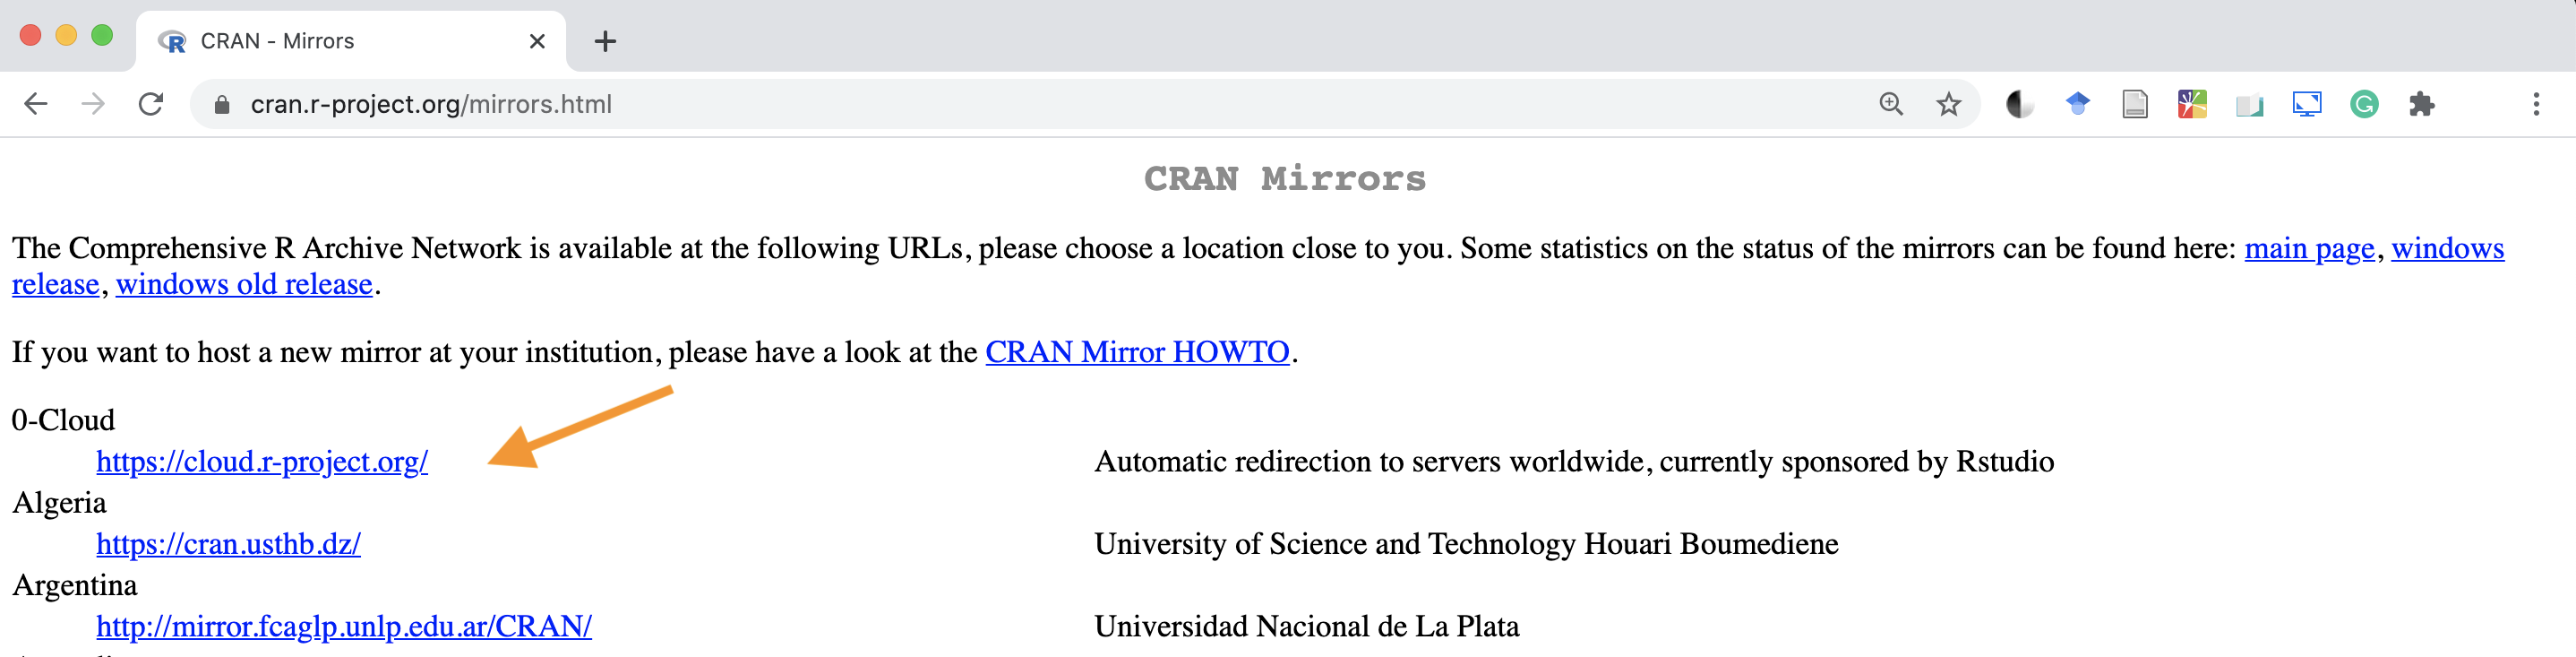
\includegraphics[width=0.95\textwidth,height=\textheight]{images/install_mirror.png}

\begin{enumerate}
\def\labelenumi{\arabic{enumi}.}
\setcounter{enumi}{3}
\tightlist
\item
  Selezionare il proprio sistema operativo
\end{enumerate}

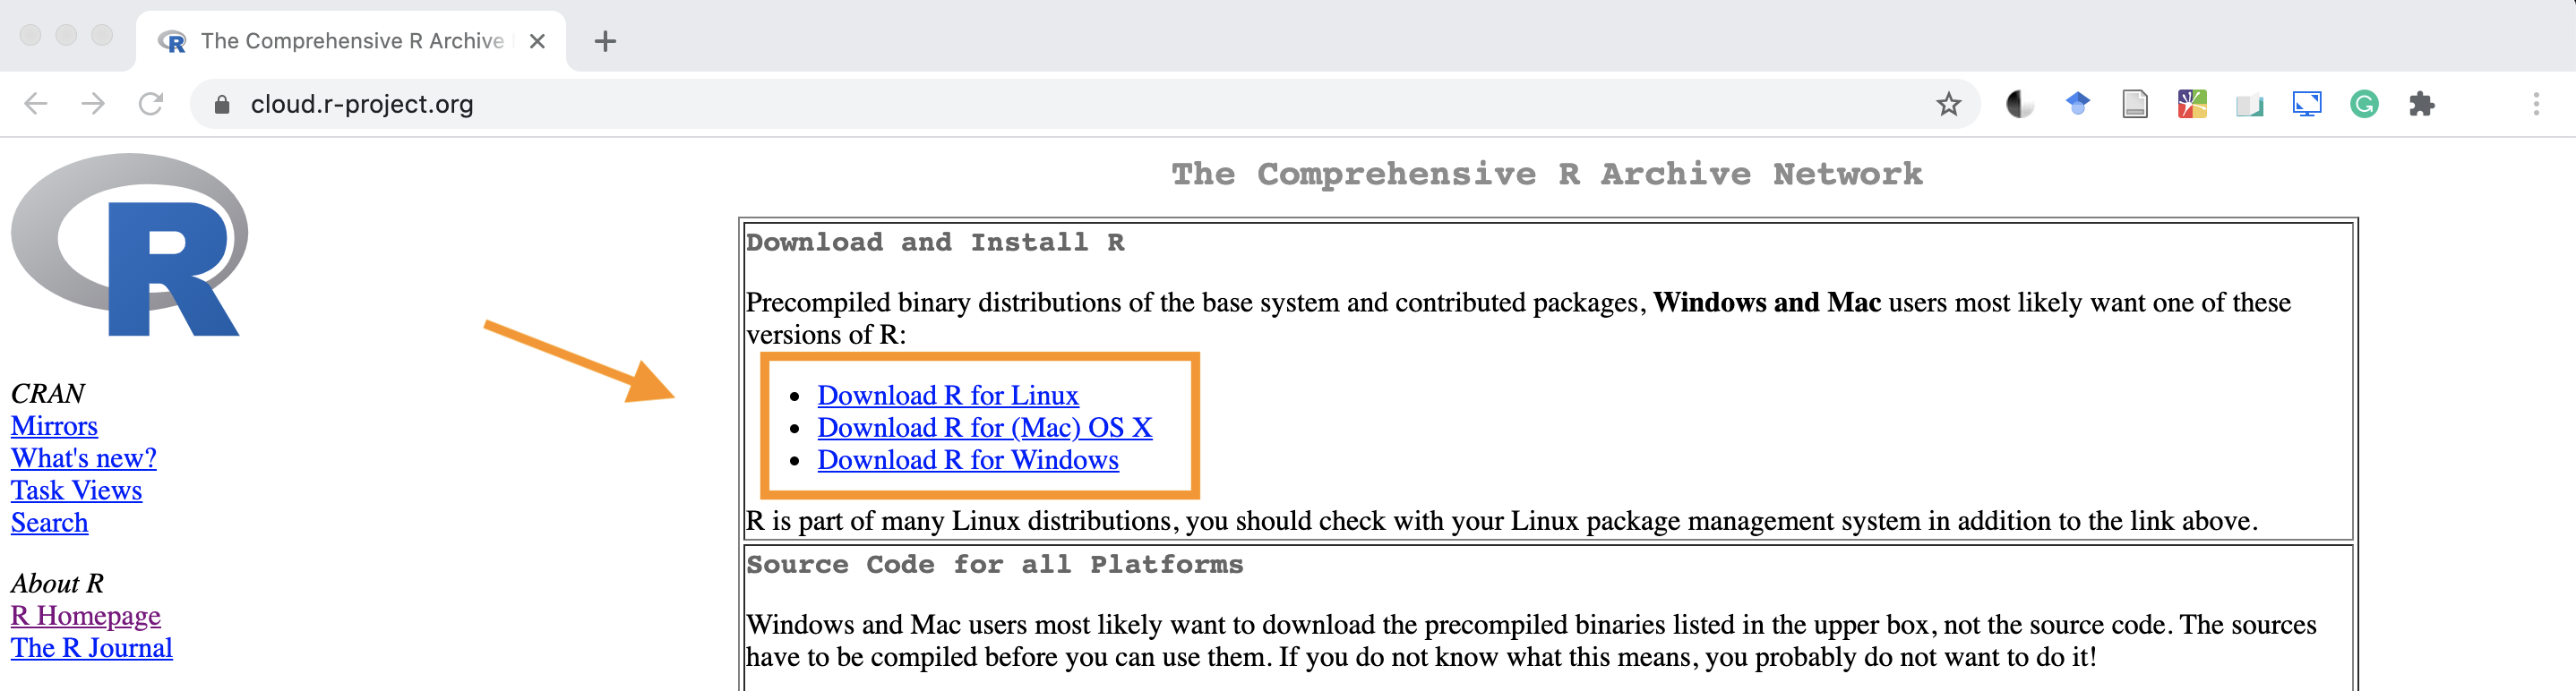
\includegraphics[width=0.95\textwidth,height=\textheight]{images/install_OS.png}

\hypertarget{r-windows}{%
\subsection{R Windows}\label{r-windows}}

\begin{enumerate}
\def\labelenumi{\arabic{enumi}.}
\tightlist
\item
  Selezionare la voce \textbf{base}
\end{enumerate}

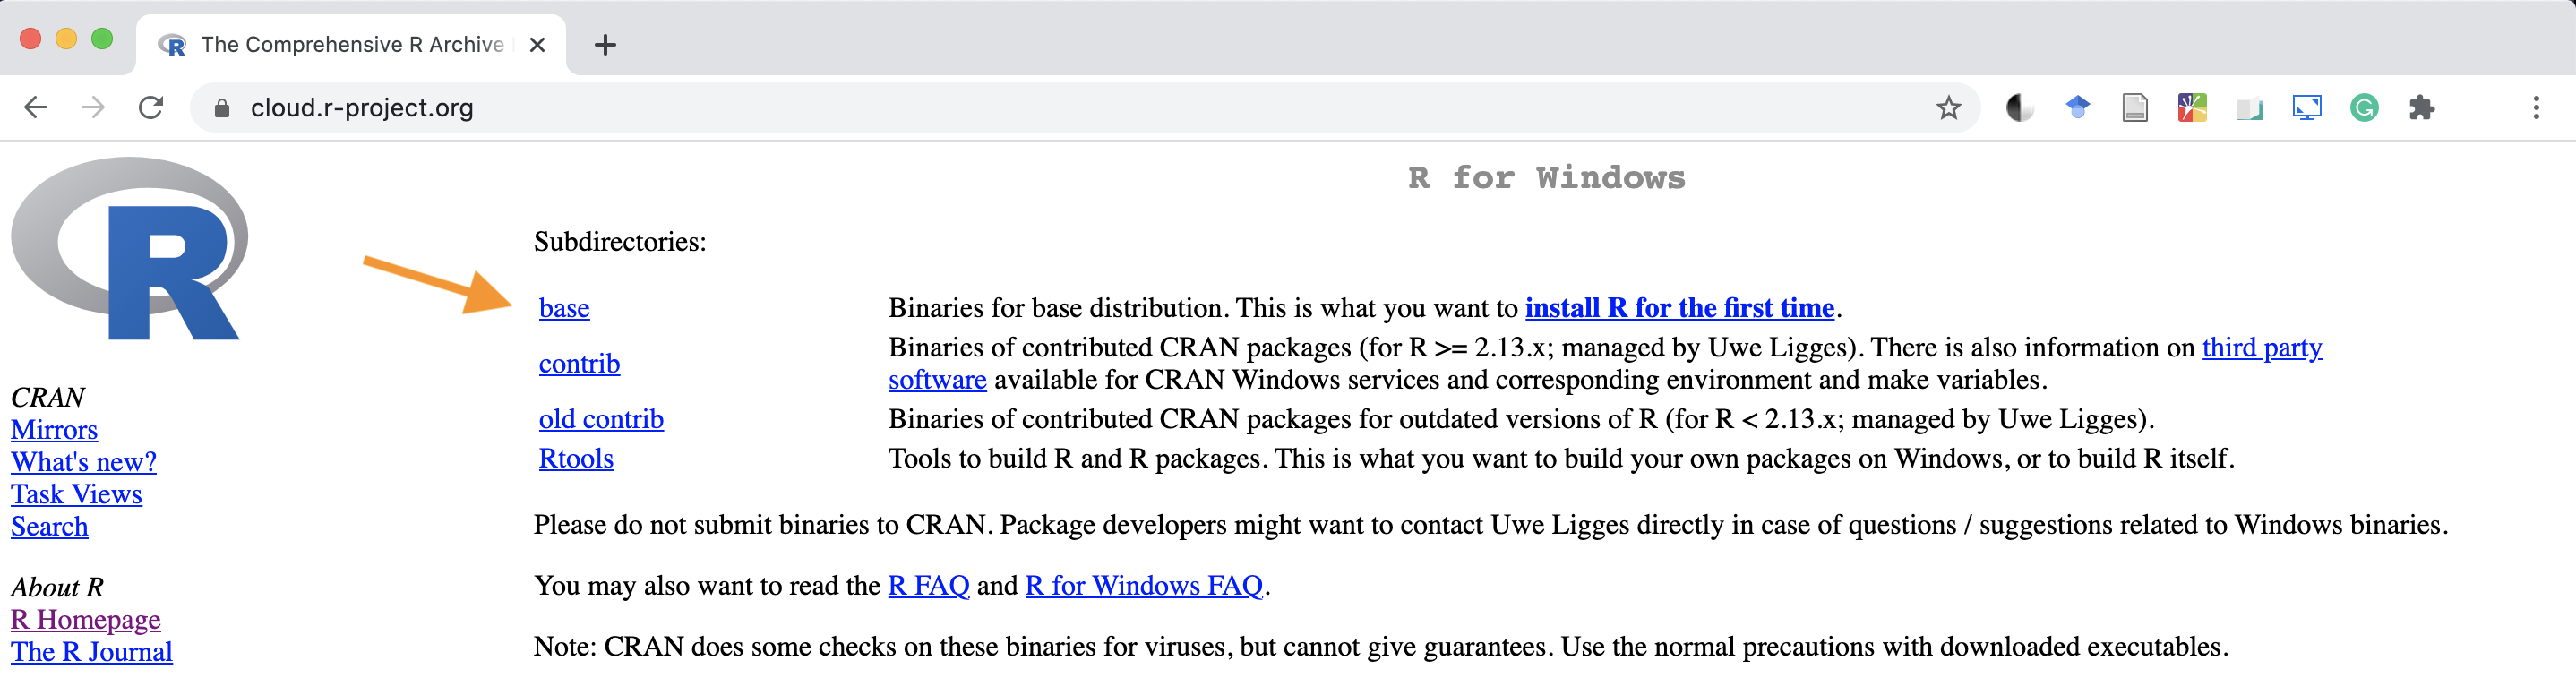
\includegraphics[width=0.95\textwidth,height=\textheight]{images/install-Windows-base.png}

\begin{enumerate}
\def\labelenumi{\arabic{enumi}.}
\setcounter{enumi}{1}
\tightlist
\item
  Selezionare la voce \textbf{Download} della versione più recente di R disponibile
\end{enumerate}

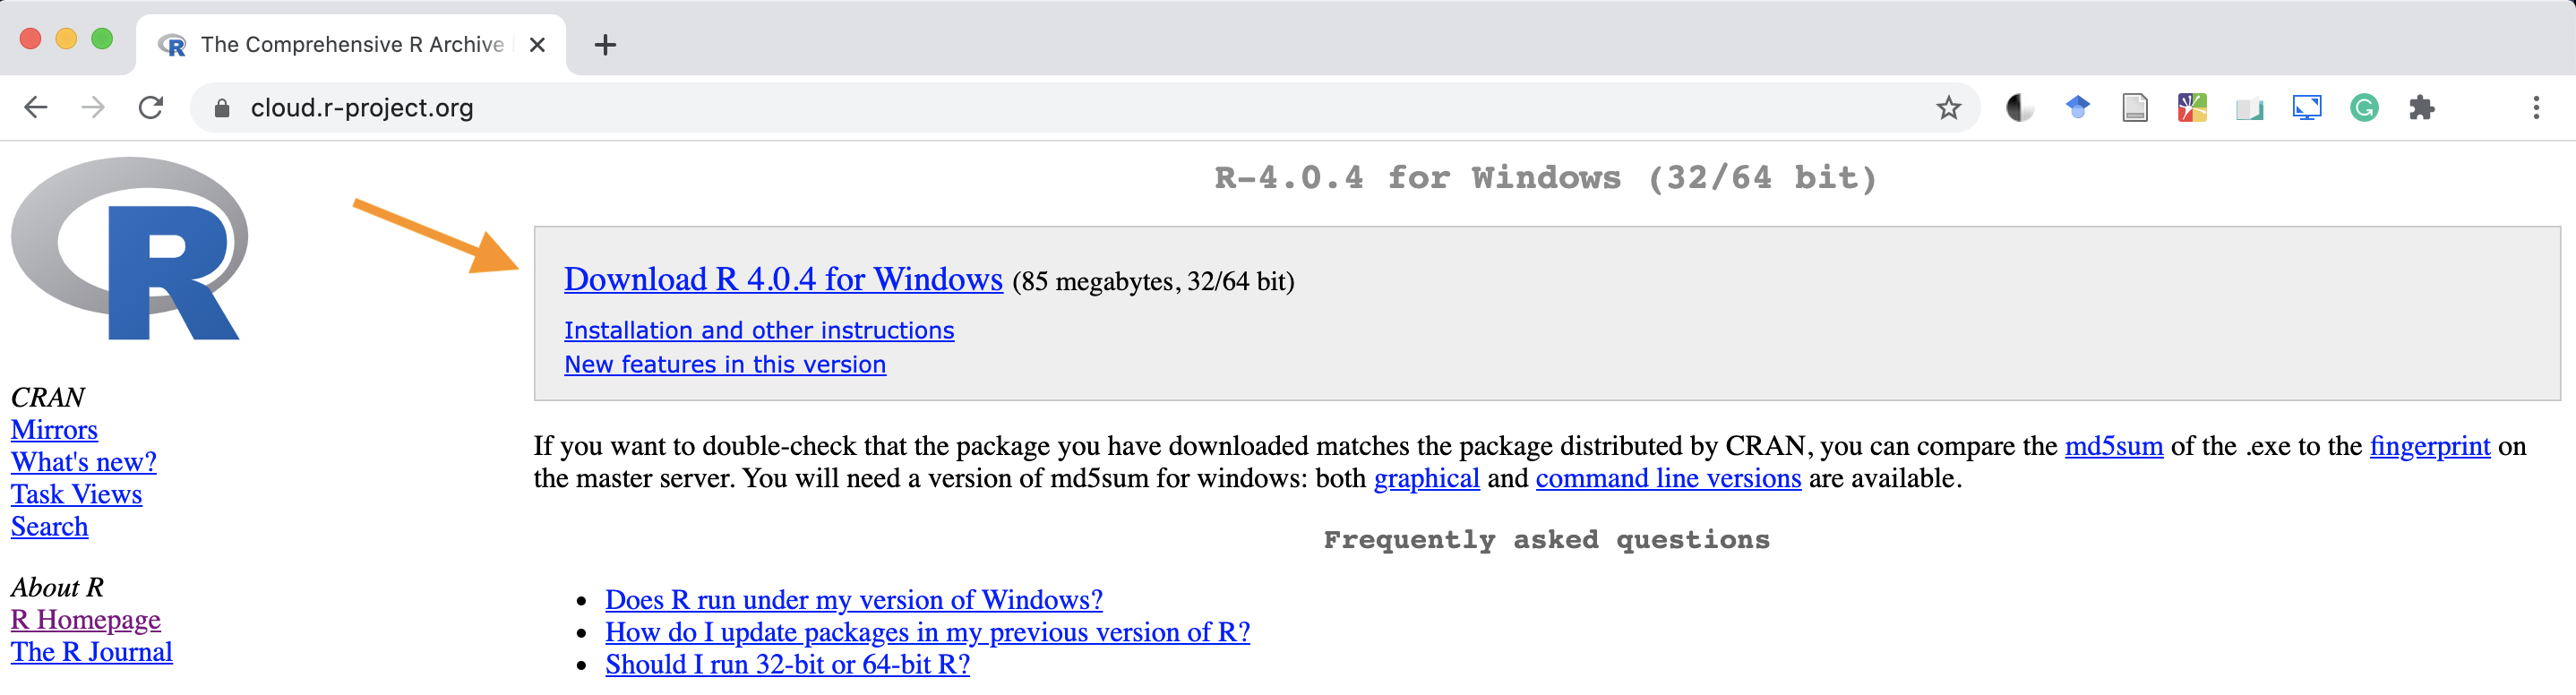
\includegraphics[width=0.95\textwidth,height=\textheight]{images/install-Windows-version.png}

\begin{enumerate}
\def\labelenumi{\arabic{enumi}.}
\setcounter{enumi}{2}
\tightlist
\item
  Al termine del download, eseguire il file e seguire le istruzioni fino al termine dell'installazione
\end{enumerate}

\hypertarget{r-macos}{%
\subsection{R MacOS}\label{r-macos}}

\begin{enumerate}
\def\labelenumi{\arabic{enumi}.}
\tightlist
\item
  Selezionare della versione più recente di R disponibile
\end{enumerate}

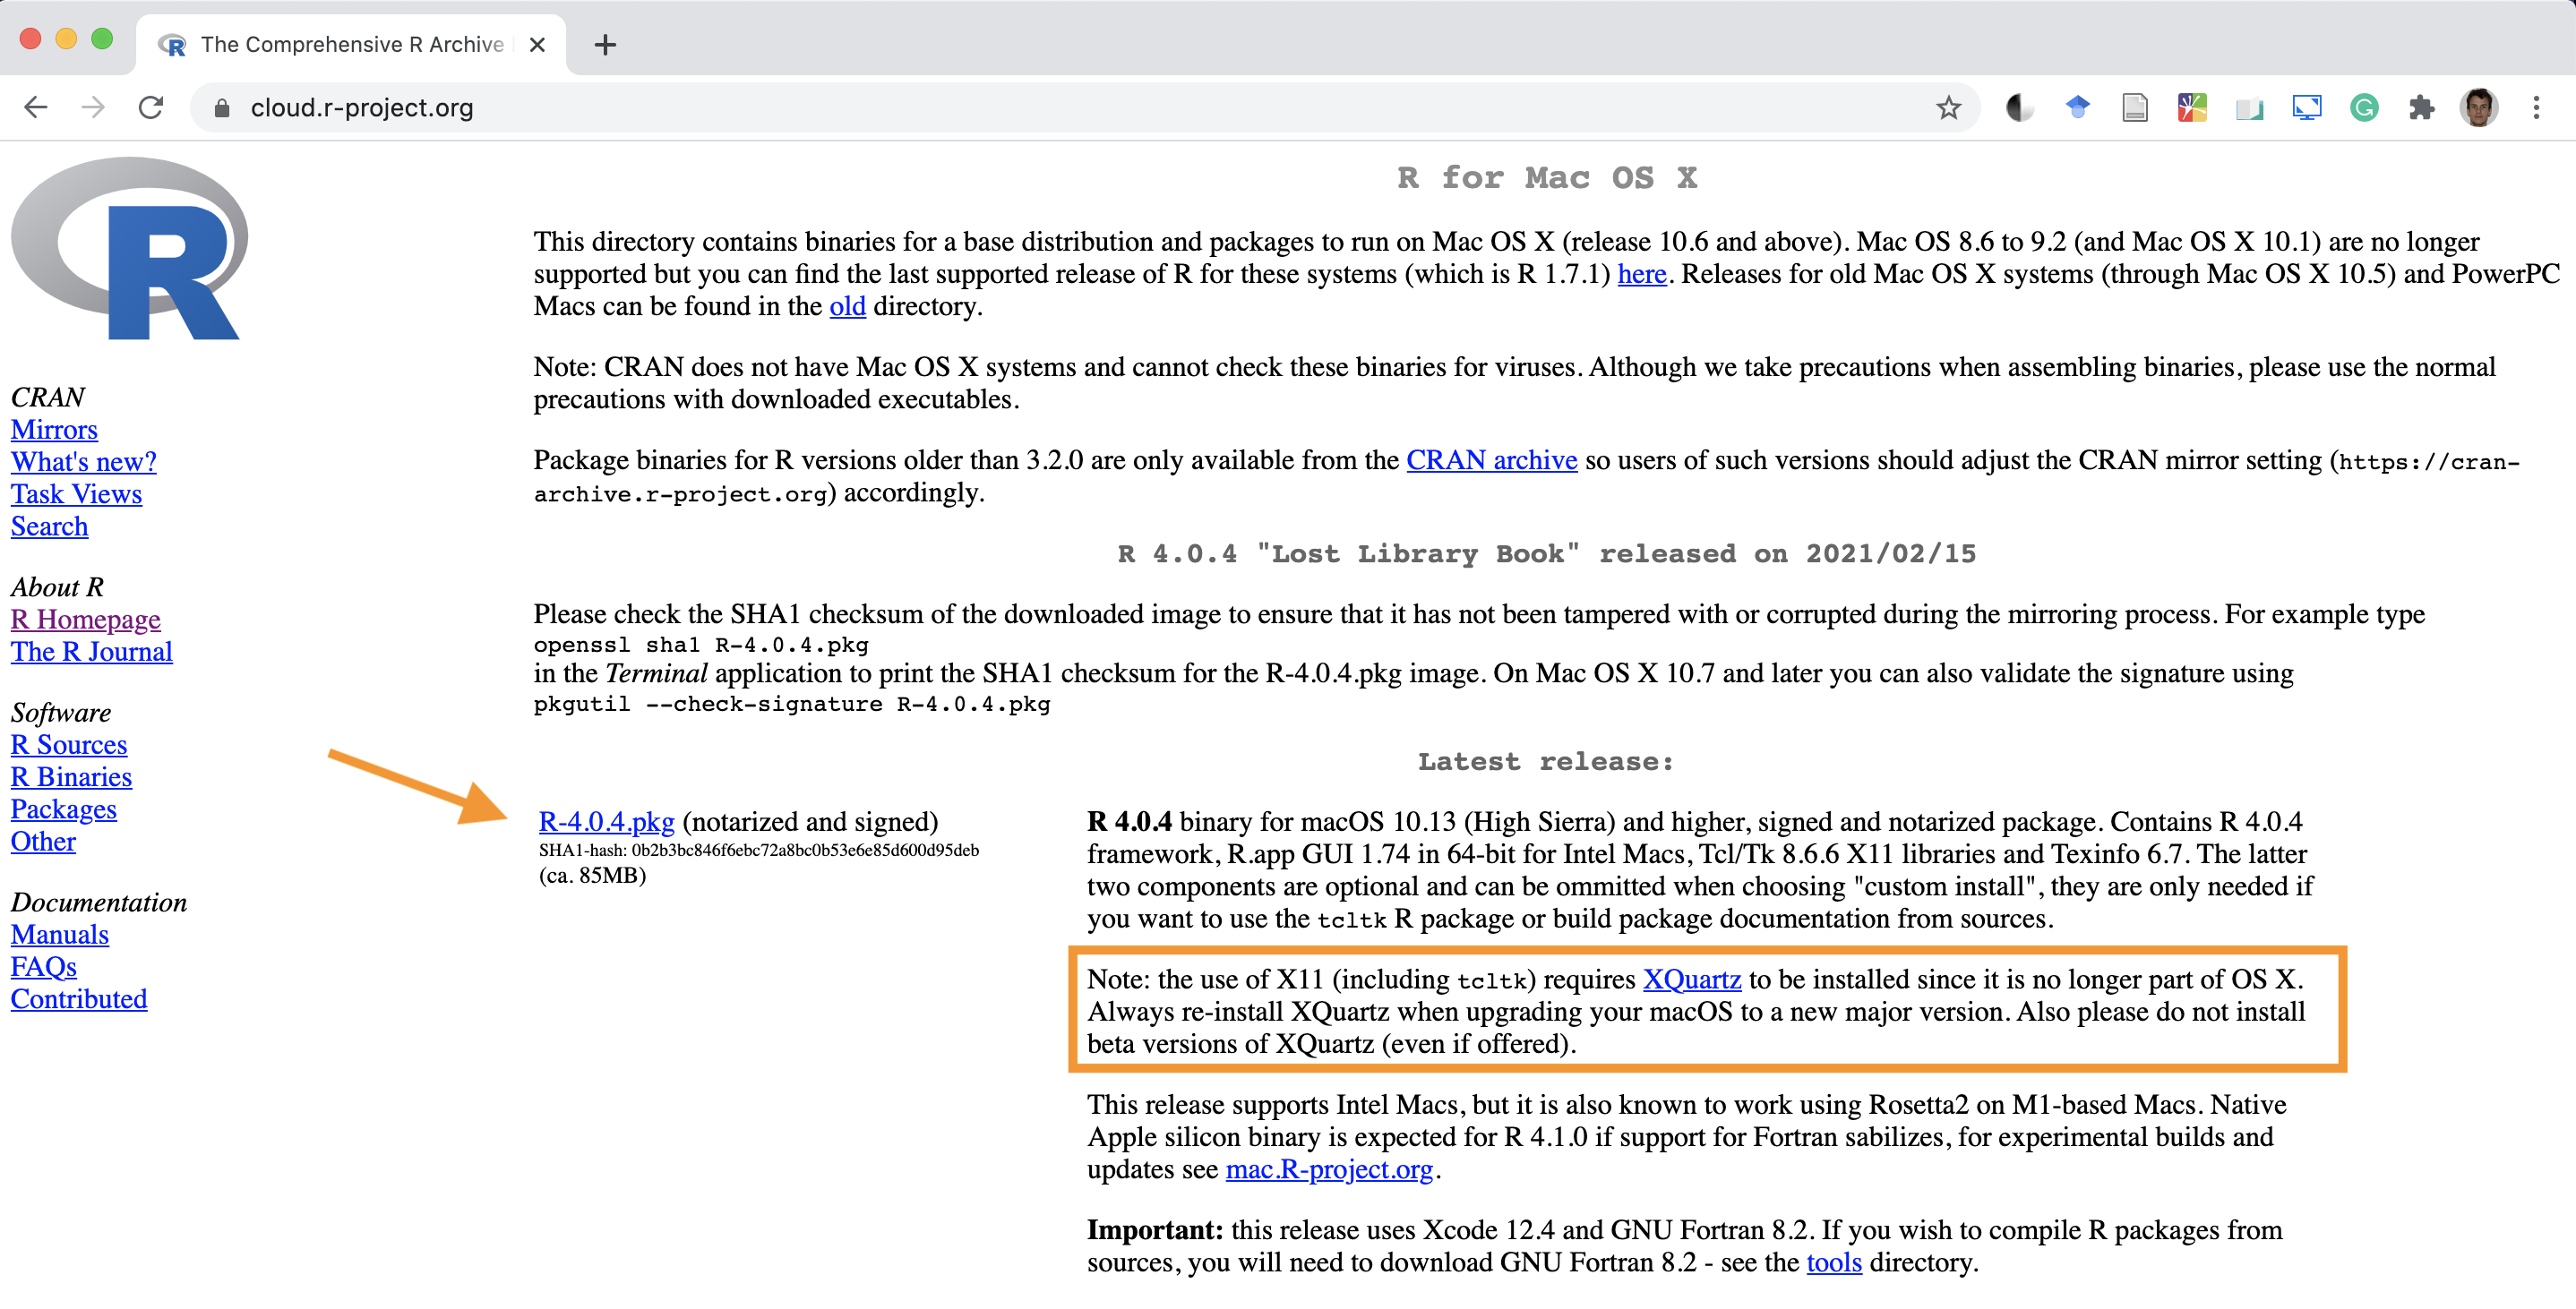
\includegraphics[width=0.95\textwidth,height=\textheight]{images/install_Mac_version.png}

\begin{enumerate}
\def\labelenumi{\arabic{enumi}.}
\setcounter{enumi}{1}
\tightlist
\item
  Al termine del download, eseguire il file e seguire le istruzioni fino al termine dell'installazione di R
\item
  Successivamente è necessario installare anche una componente aggiuntiva \textbf{XQuartz} premendo il link all'interno del riquadro arancione riportato nella figura precedente
\item
  Selezionare la voce Download
\end{enumerate}

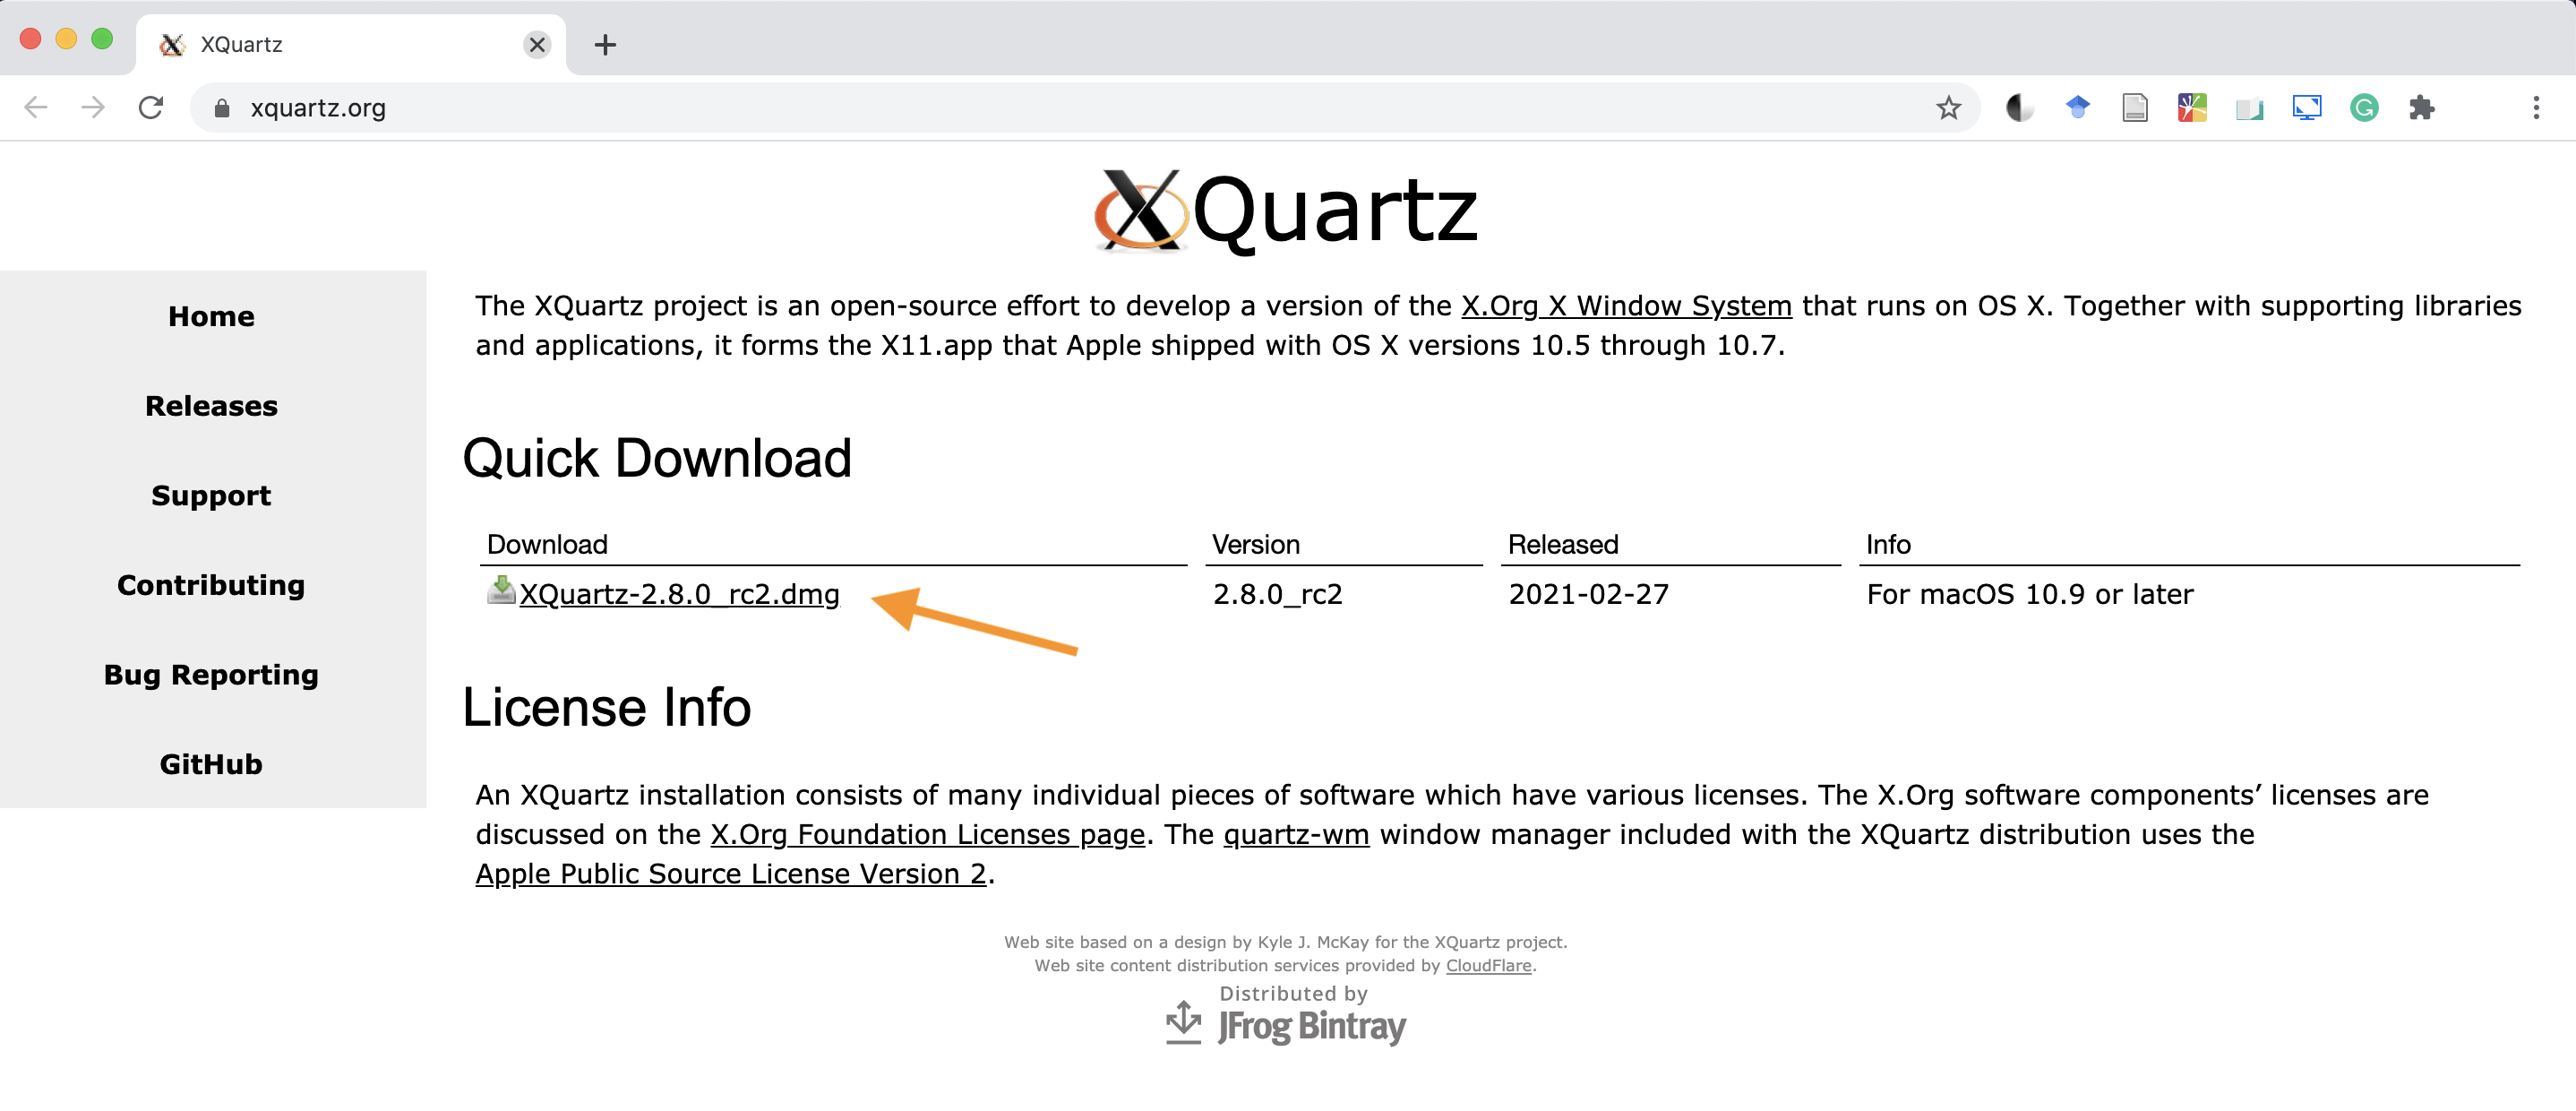
\includegraphics[width=0.95\textwidth,height=\textheight]{images/install_Mac_XQuartz.png}

\begin{enumerate}
\def\labelenumi{\arabic{enumi}.}
\setcounter{enumi}{4}
\tightlist
\item
  Al termine del download, eseguire il file e seguire le istruzioni fino al termine dell'installazione
\end{enumerate}

\begin{design}[R Tools]

Utilizzi avanzati di R richiedono l'insallazione di una serie ulteriore software definiti \textbf{R tools}.

\hypertarget{windows}{%
\subsubsection*{Windows}\label{windows}}
\addcontentsline{toc}{subsubsection}{Windows}

Seleziona la voce \textbf{Rtools} e segui le istruzioni per completare l'installazione.

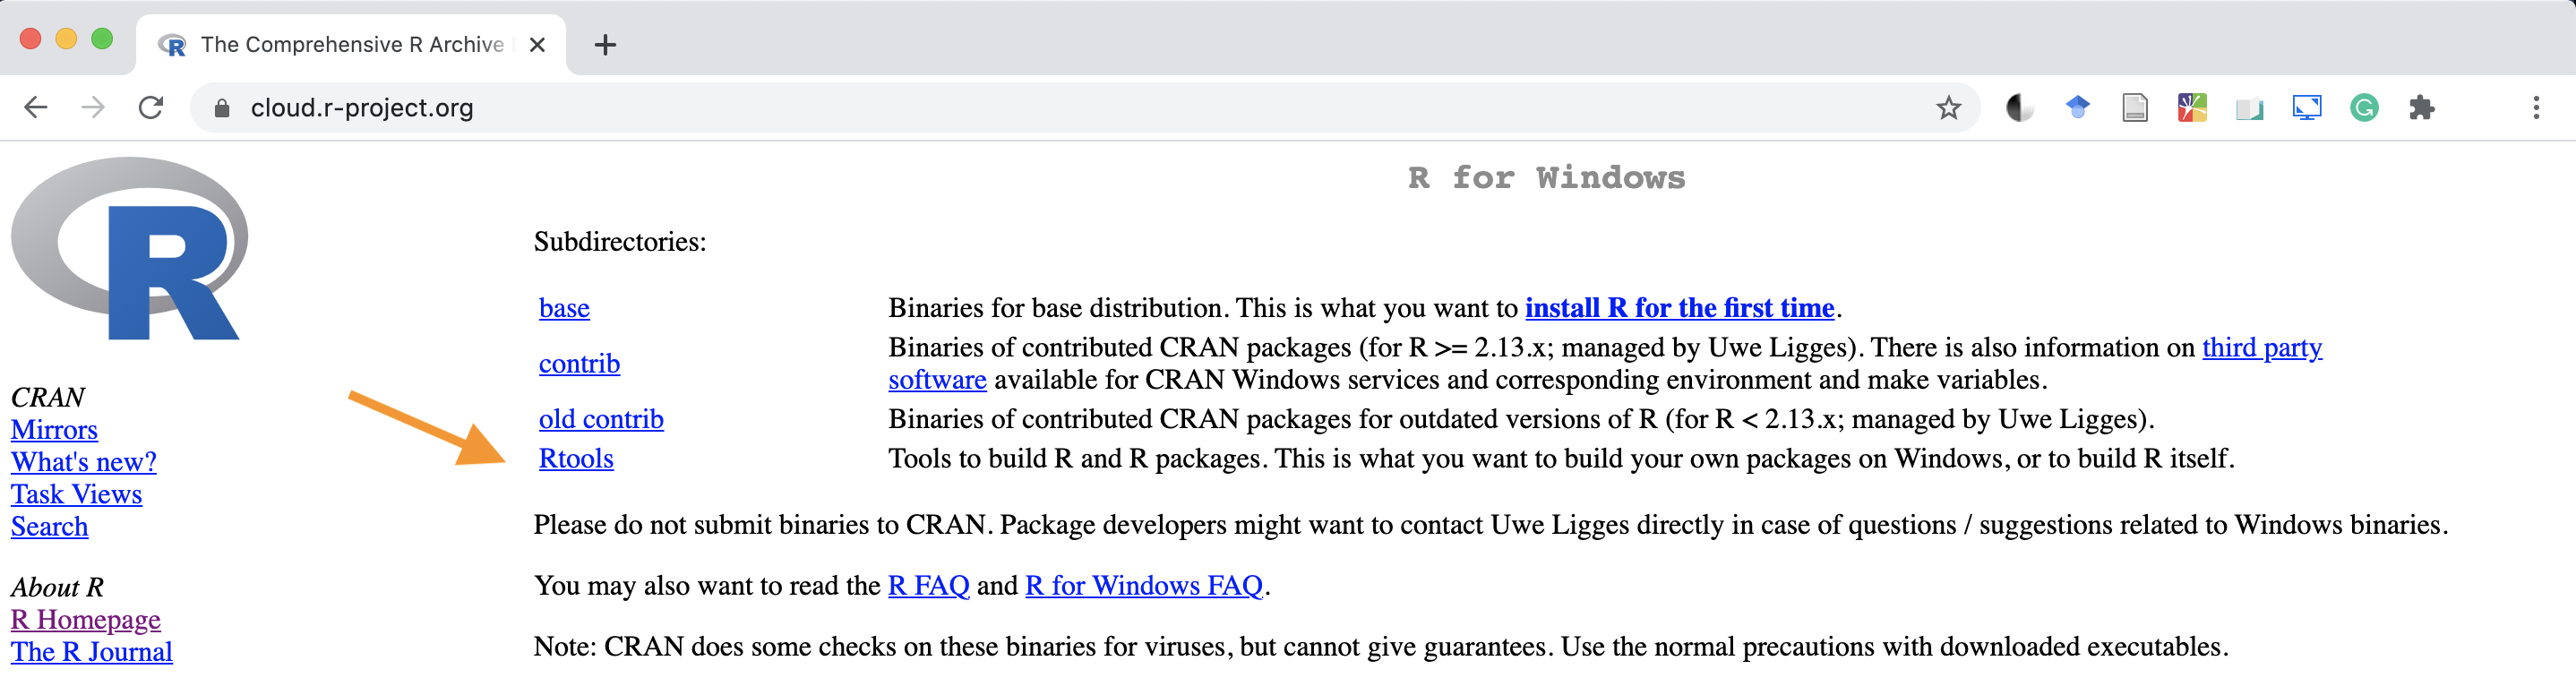
\includegraphics[width=0.95\textwidth,height=\textheight]{images/install-Windows-tools.png}

Nota che sono richieste anche delle operazioni di configurazione affinchè tutto funzioni correttamente.

\hypertarget{macos}{%
\subsubsection*{MacOS}\label{macos}}
\addcontentsline{toc}{subsubsection}{MacOS}

Seleziona la voce \textbf{tools} e segui le istruzioni riportate.

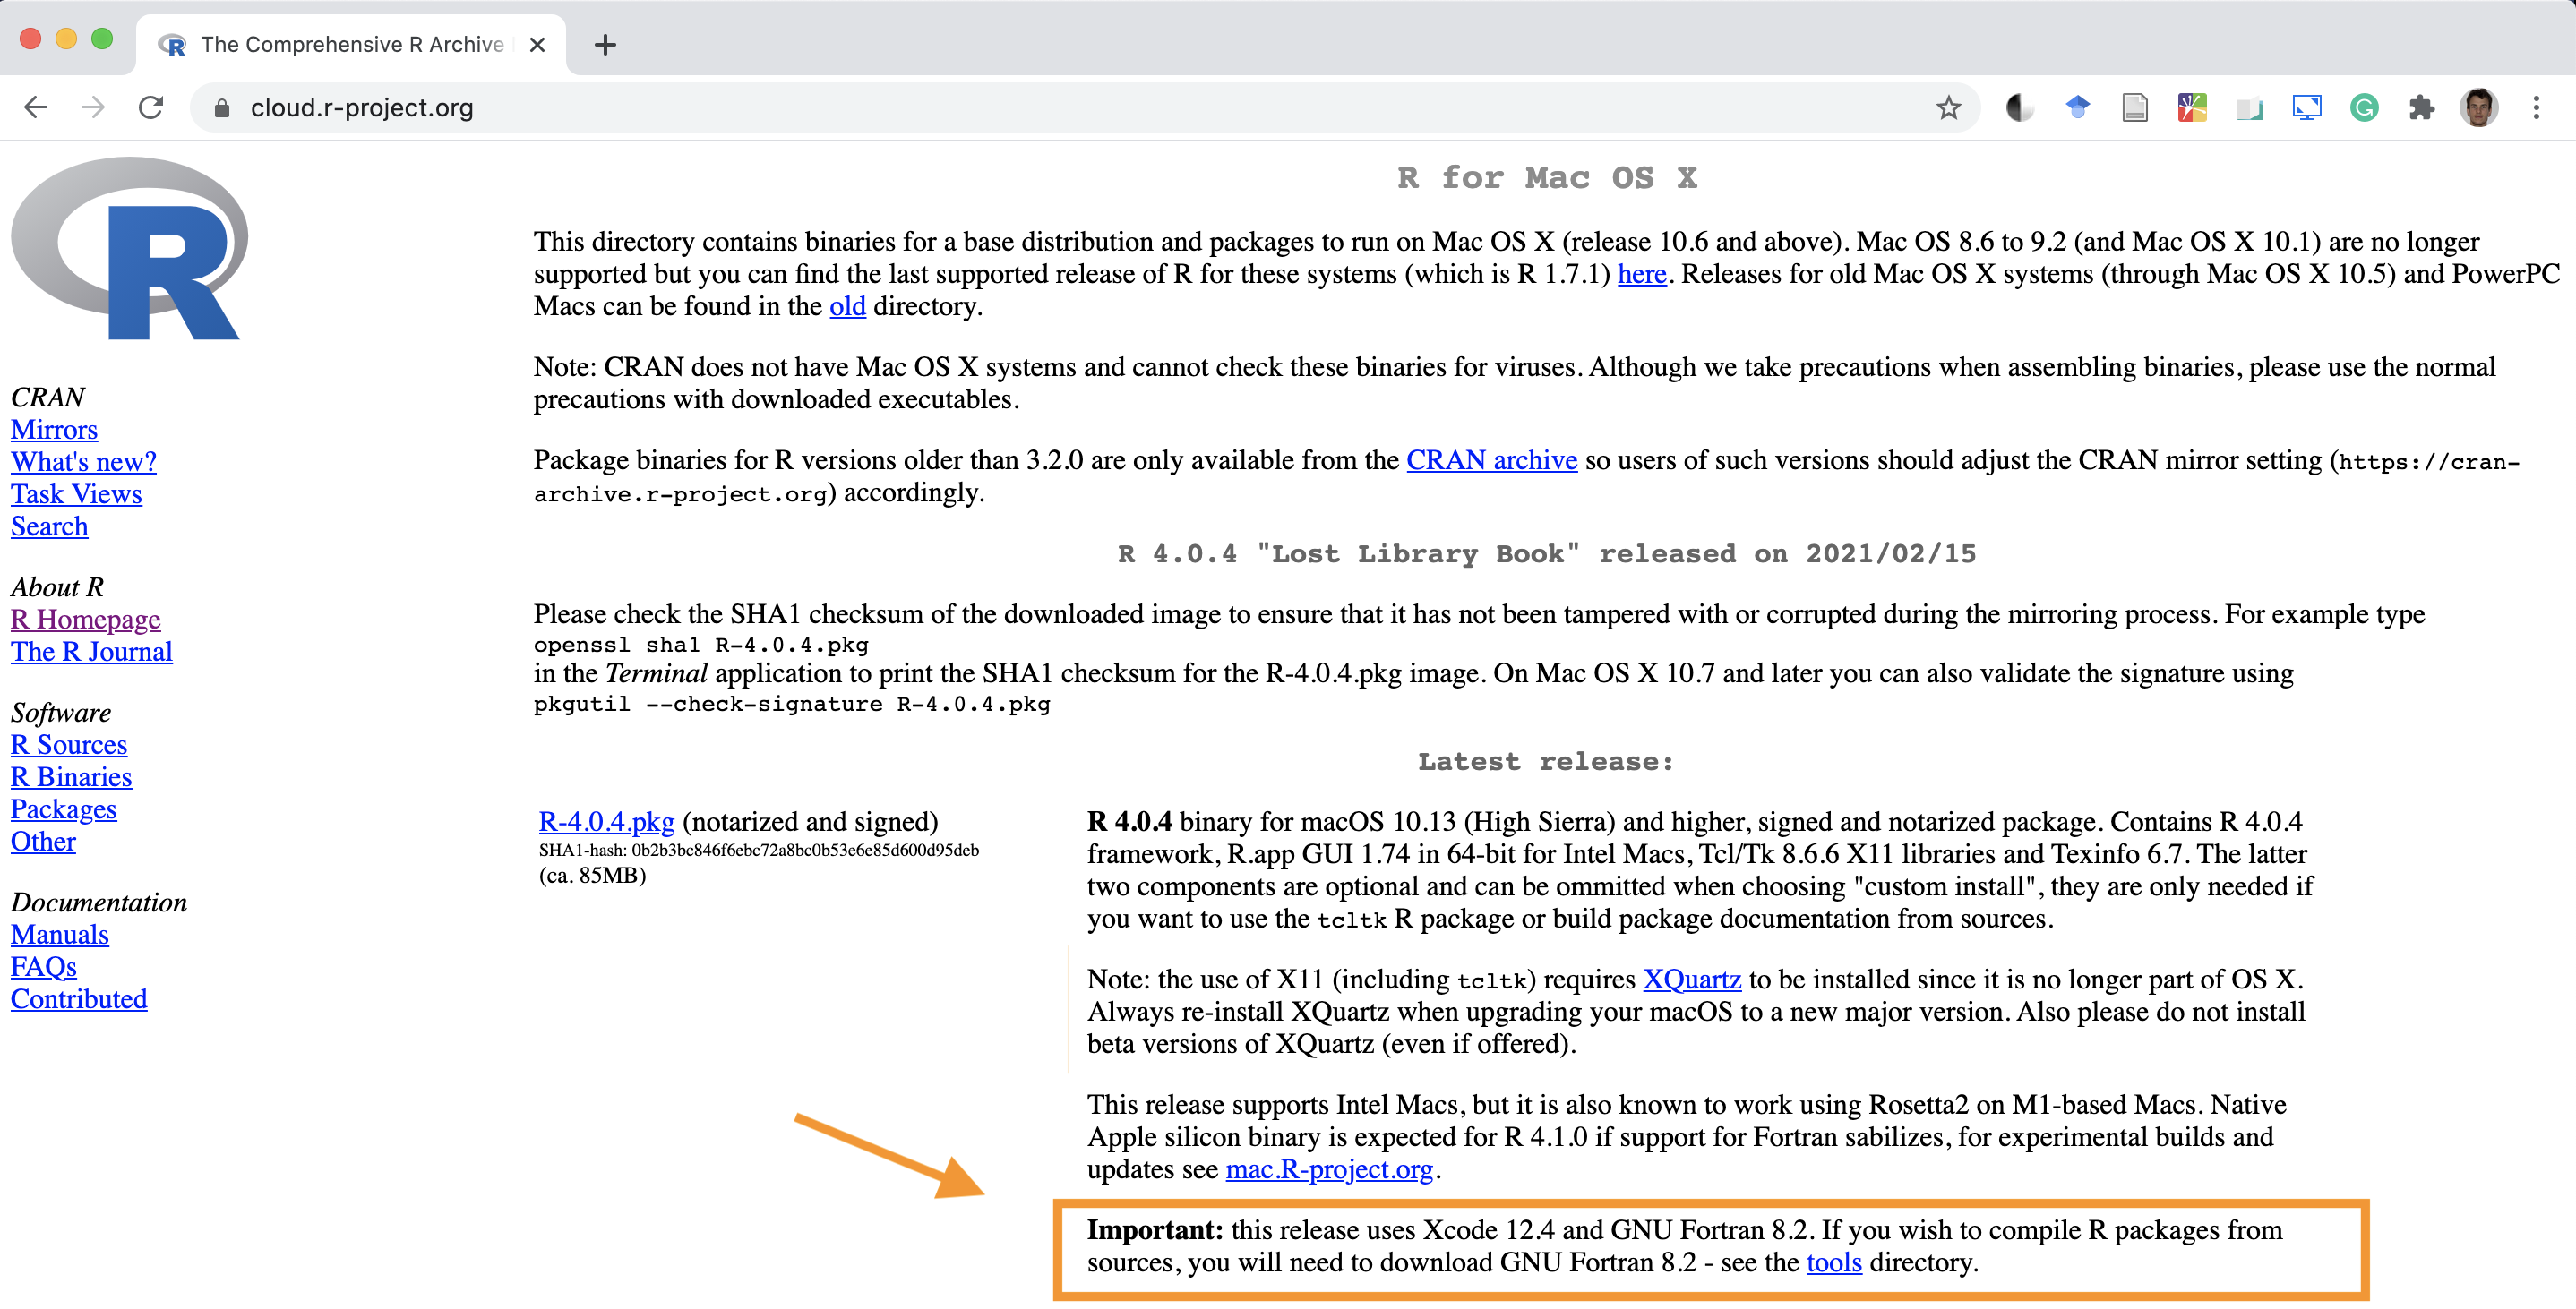
\includegraphics[width=0.95\textwidth,height=\textheight]{images/install_Mac_tools.png}

Nota in particolare che con R 4.0 le seguenti indicazioni sono riportate.

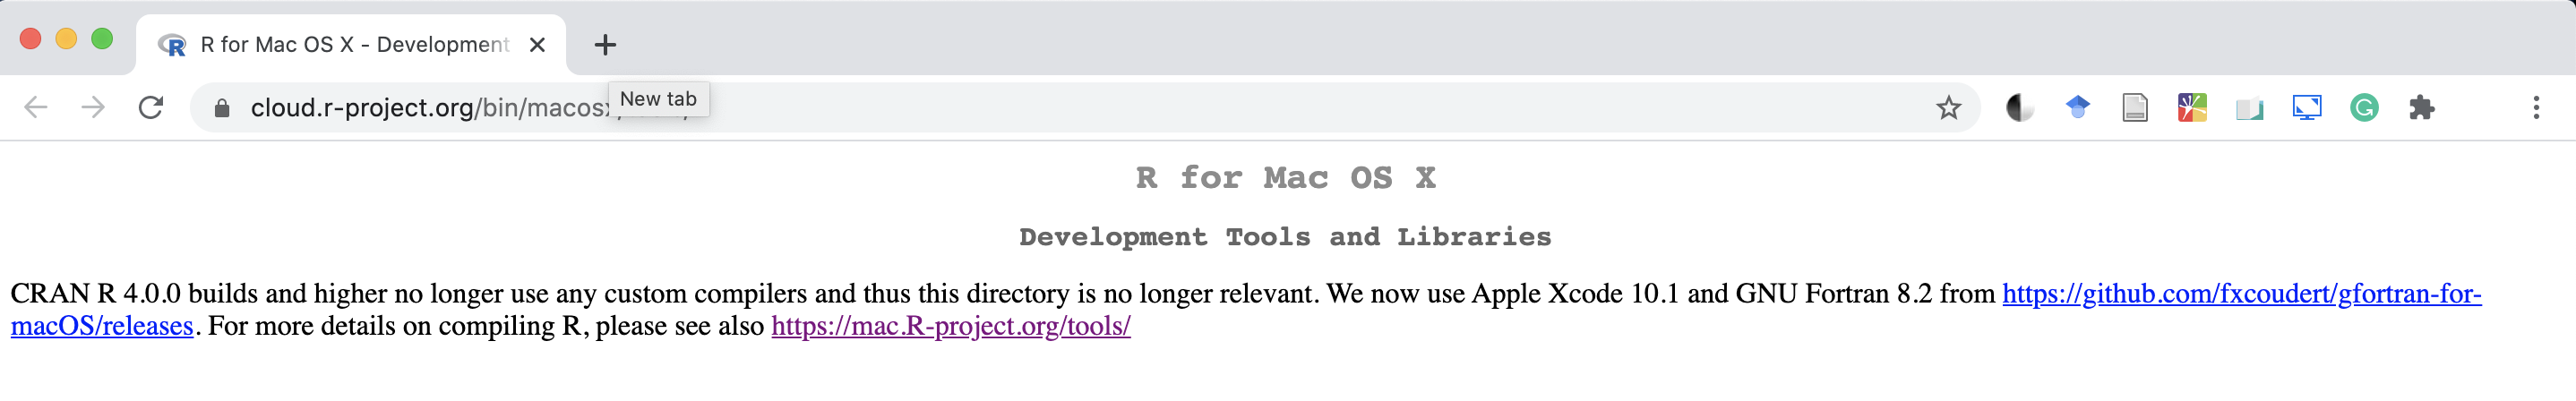
\includegraphics[width=0.95\textwidth,height=\textheight]{images/install_Mac_tools2.png}

\end{design}

\hypertarget{installare-r-studio}{%
\section{Installare R Studio}\label{installare-r-studio}}

\begin{enumerate}
\def\labelenumi{\arabic{enumi}.}
\tightlist
\item
  Accedere al sito \url{https://rstudio.com}
\item
  Selezionare la voce \textbf{DOWNLOAD IT NOW}
\end{enumerate}

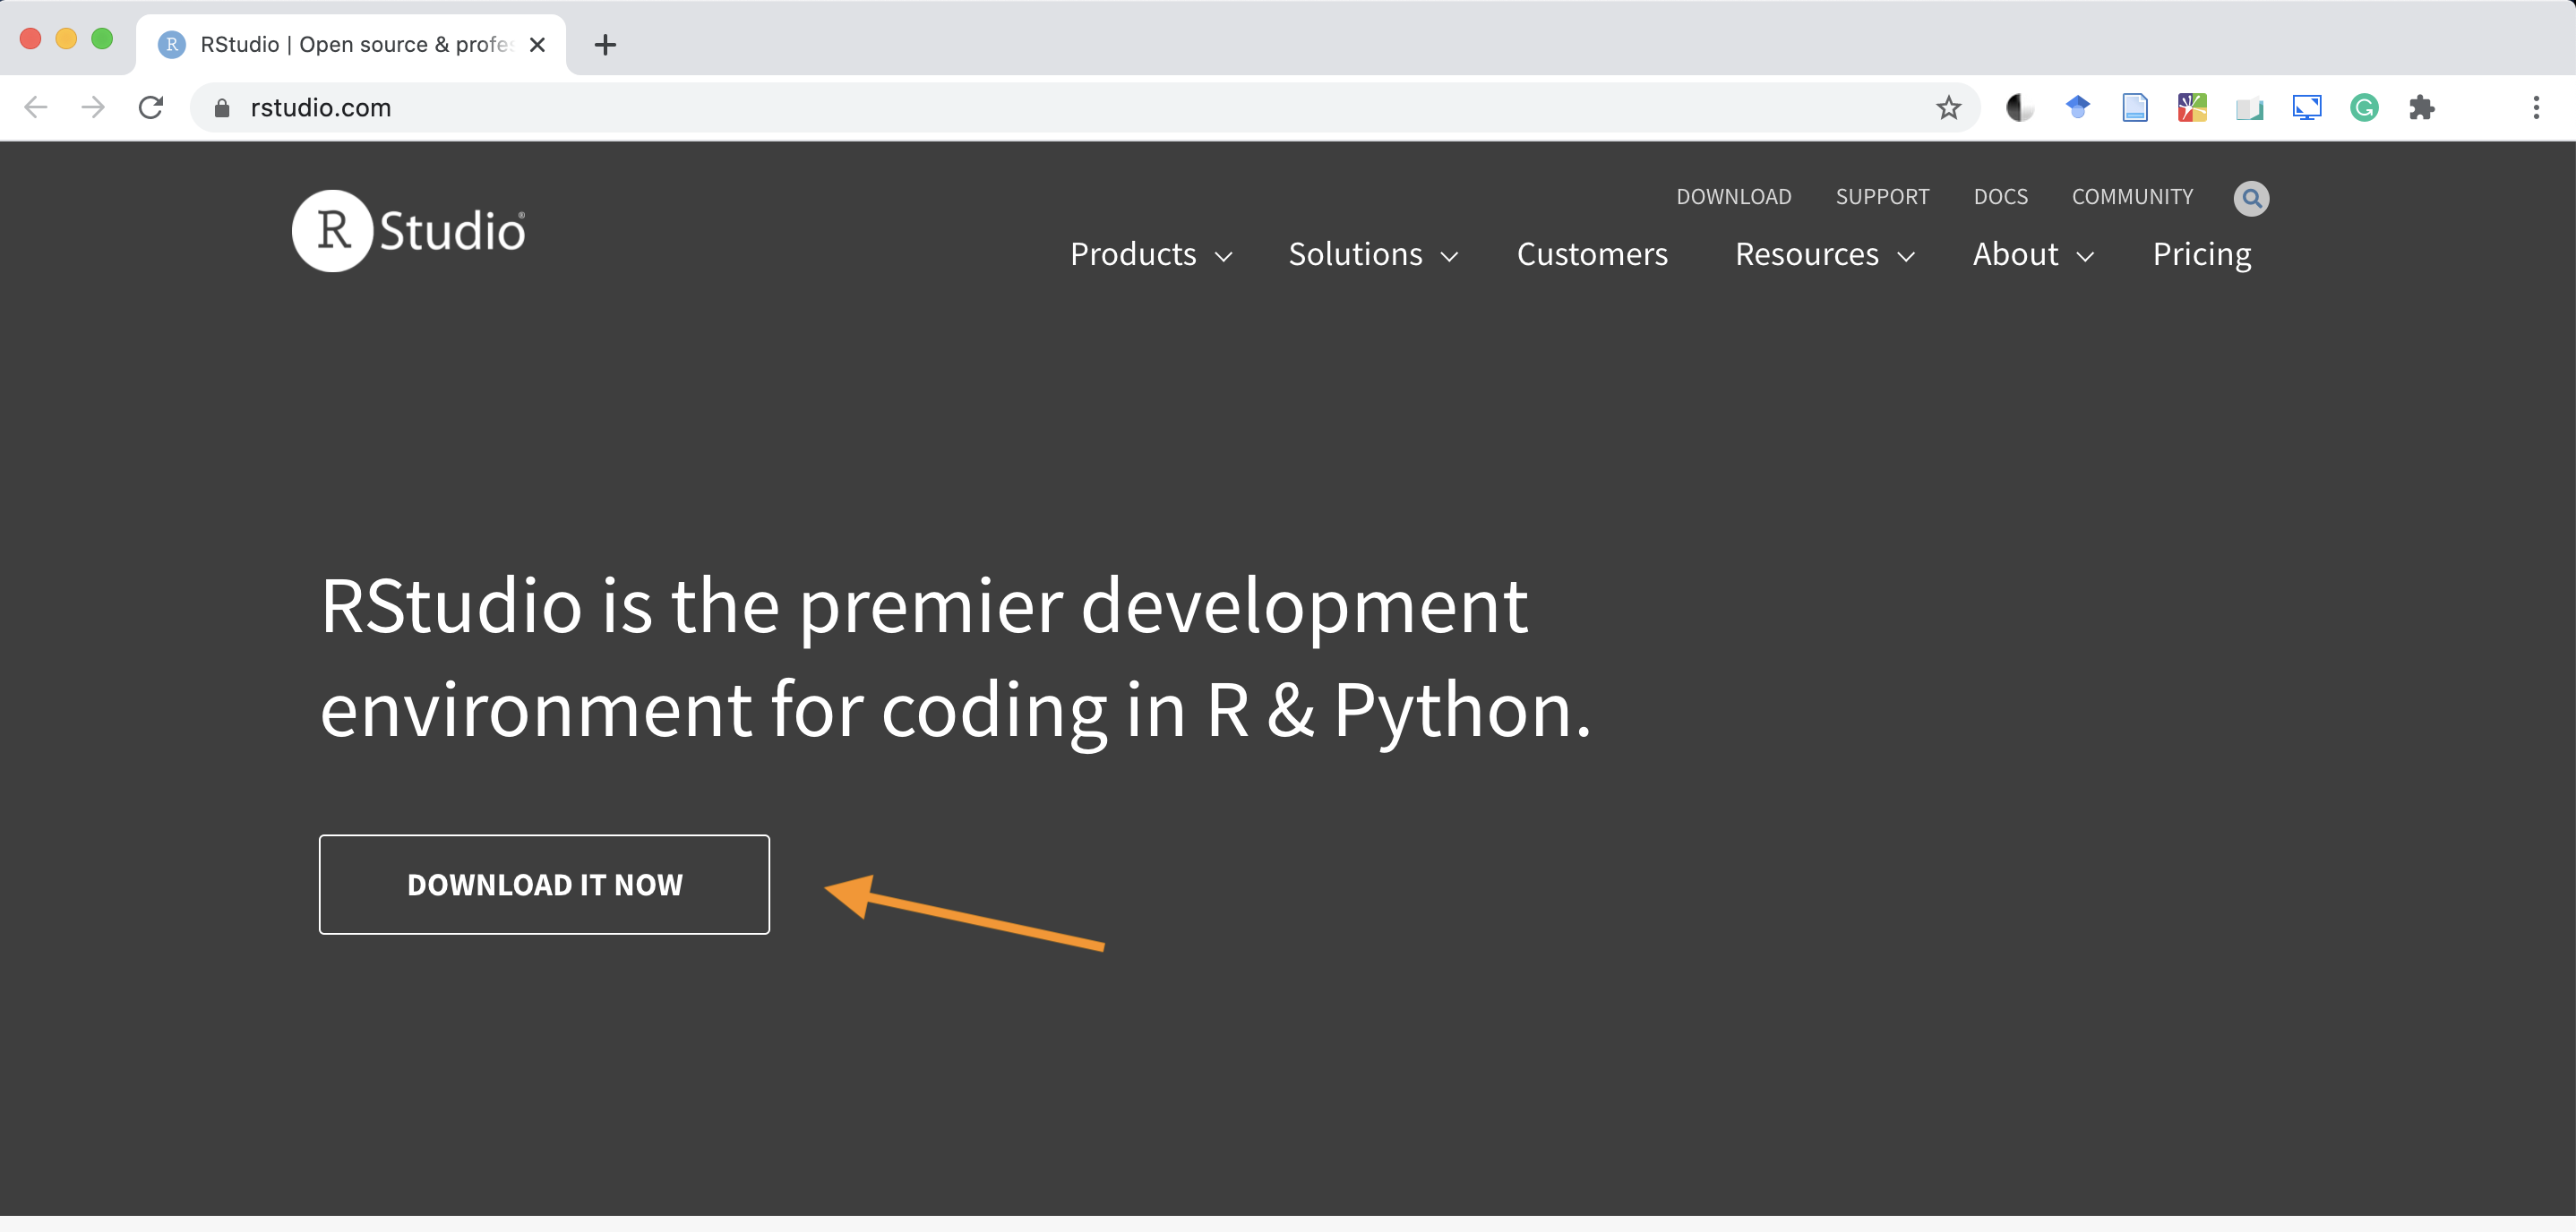
\includegraphics[width=0.95\textwidth,height=\textheight]{images/install_rstudio1.png}

\begin{enumerate}
\def\labelenumi{\arabic{enumi}.}
\setcounter{enumi}{2}
\tightlist
\item
  Selezionare la versione gratuita di RStudio Desktop
\end{enumerate}

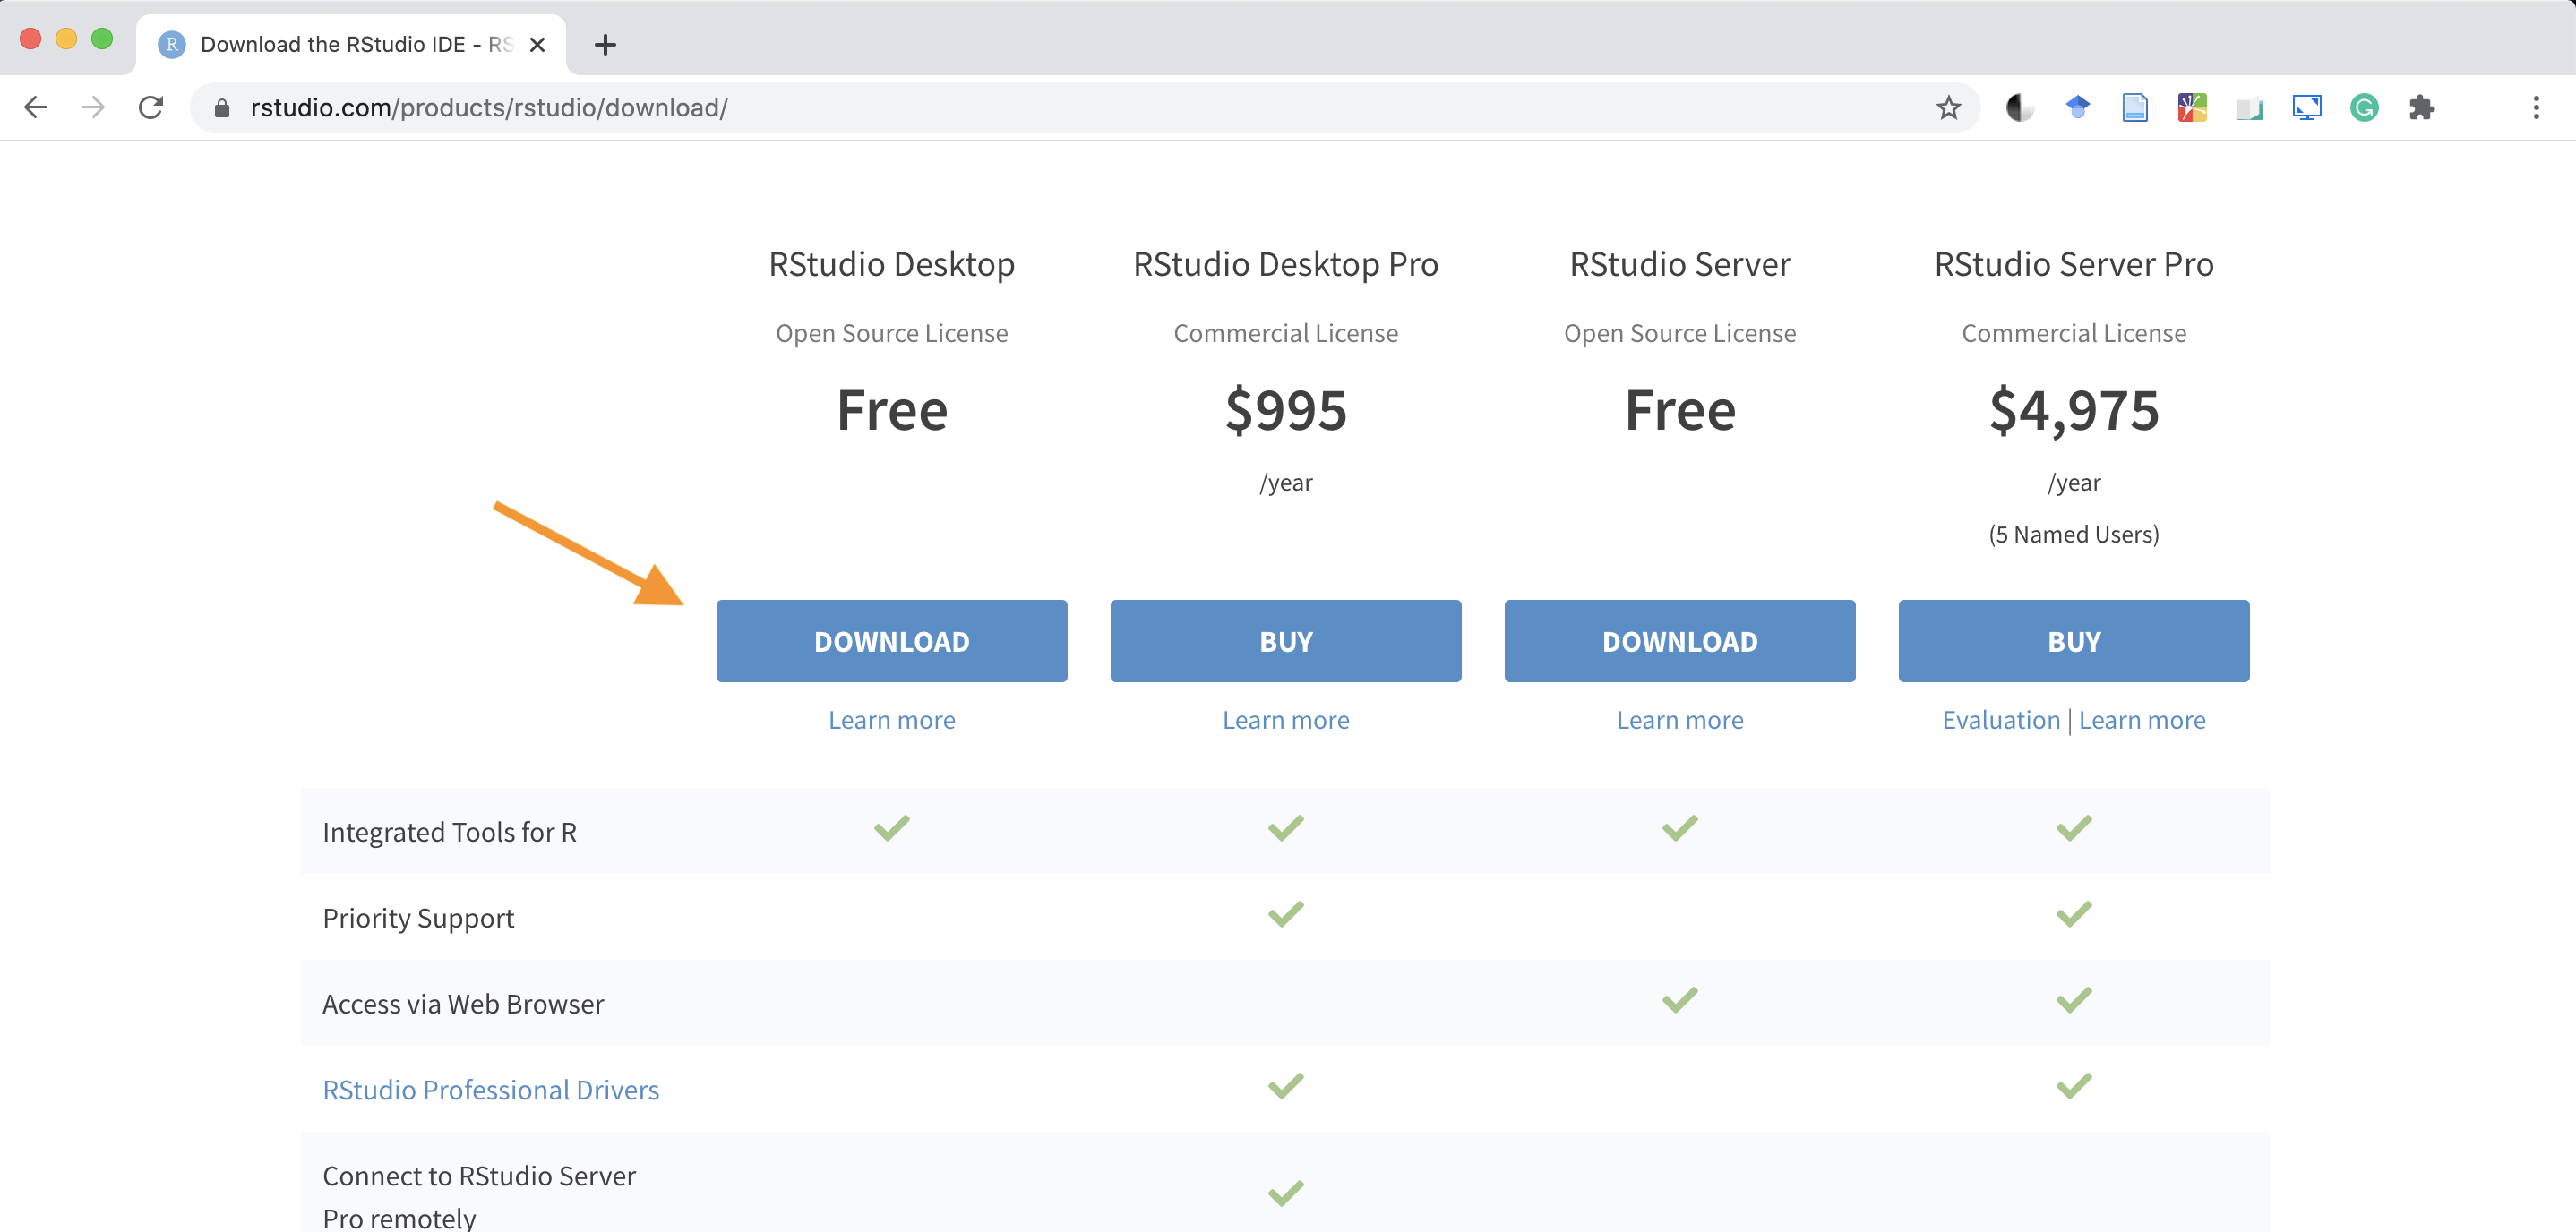
\includegraphics[width=0.95\textwidth,height=\textheight]{images/install_rstudio2.png}

\begin{enumerate}
\def\labelenumi{\arabic{enumi}.}
\setcounter{enumi}{3}
\tightlist
\item
  Selezionare la versione corretta a seconda del proprio sistema operativo
\end{enumerate}

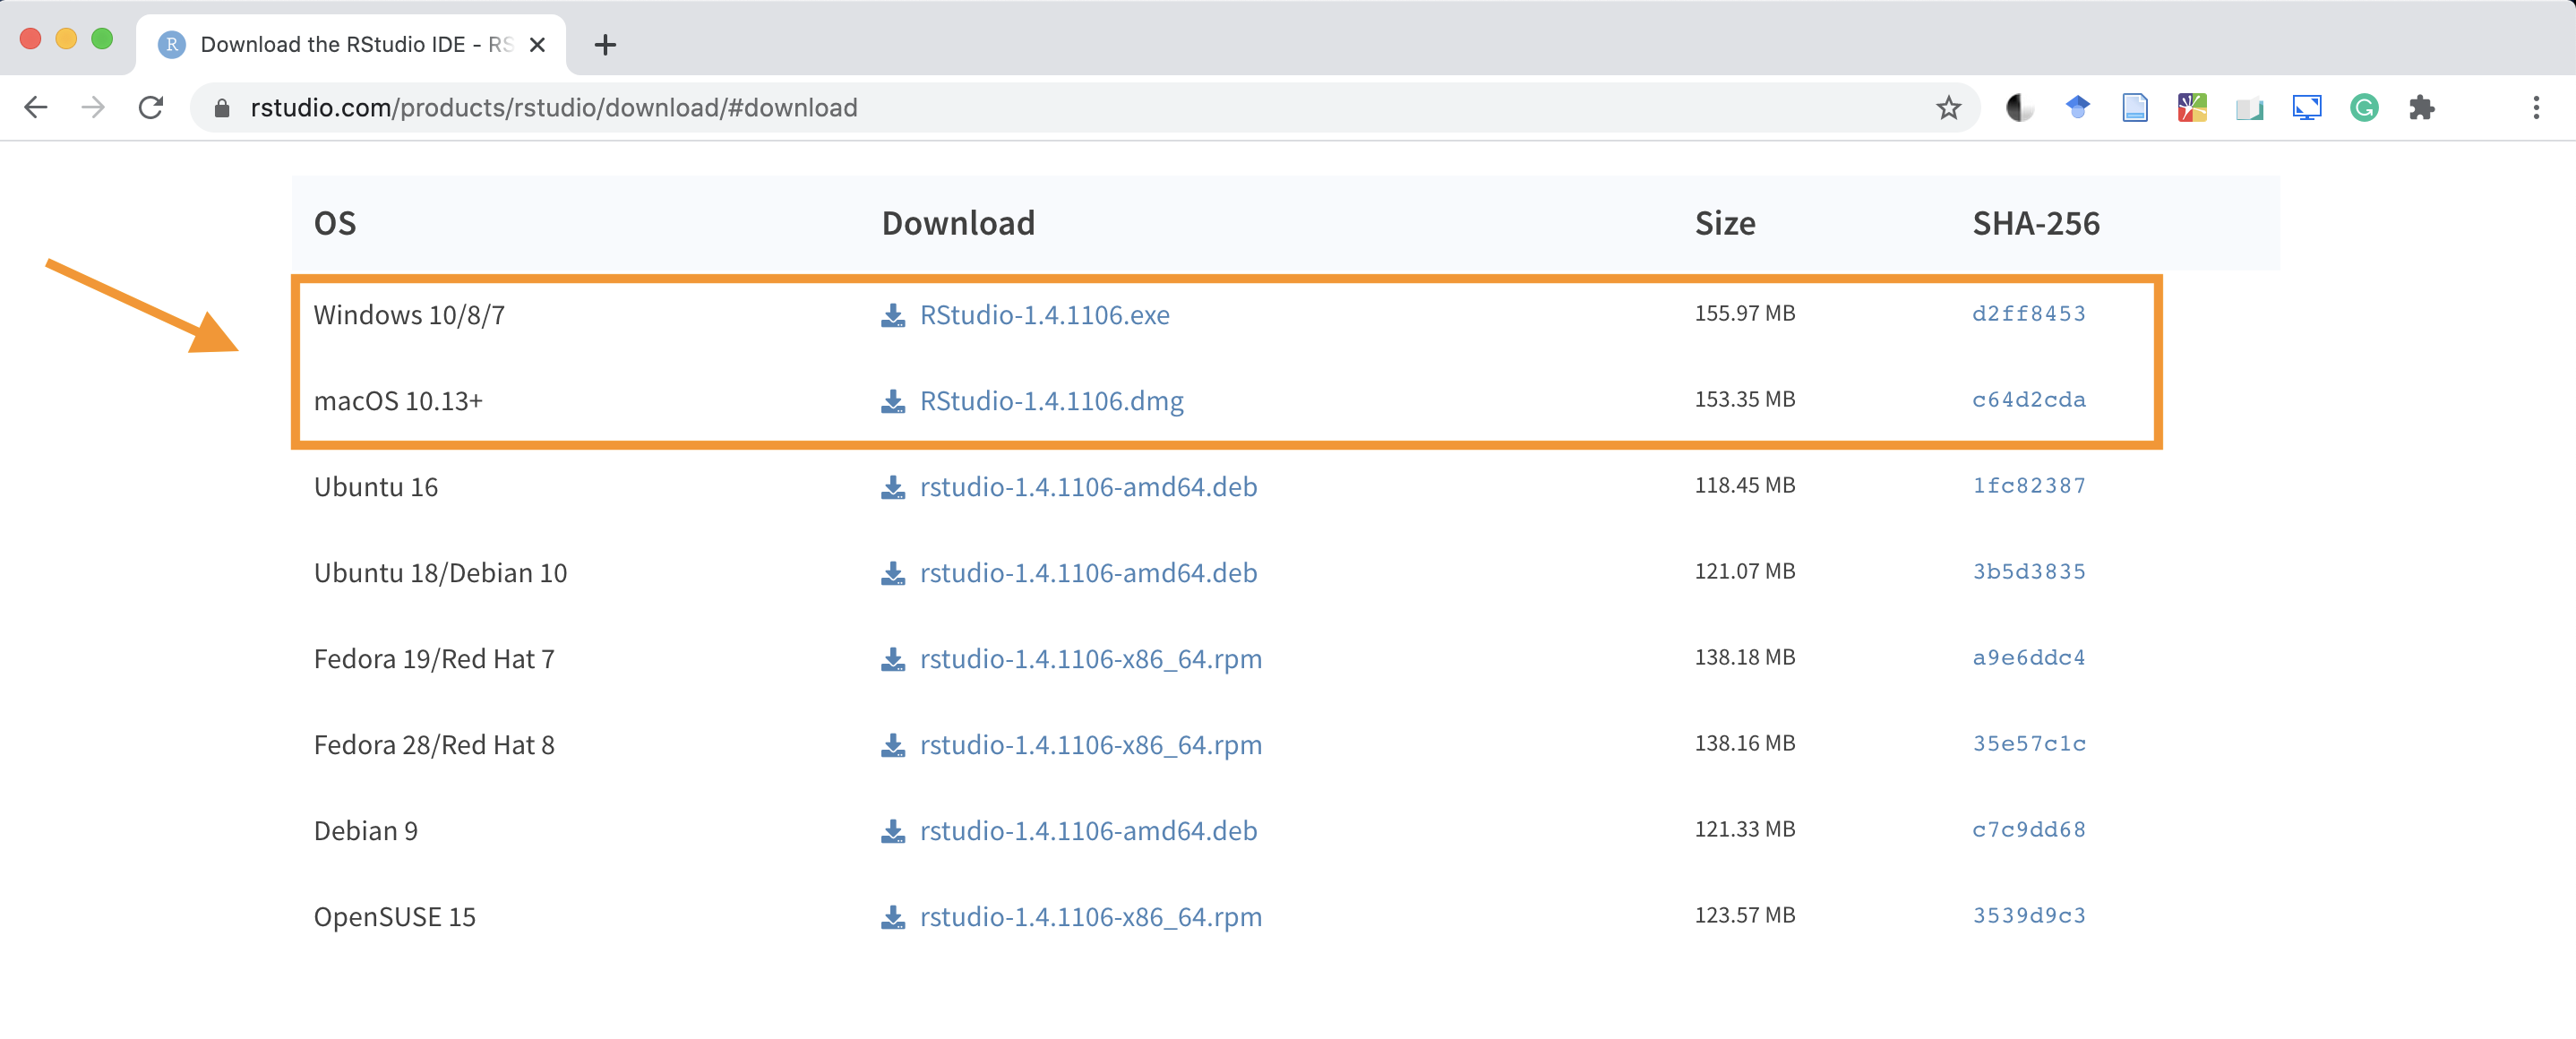
\includegraphics[width=0.95\textwidth,height=\textheight]{images/install_rstudio3.png}

\begin{enumerate}
\def\labelenumi{\arabic{enumi}.}
\setcounter{enumi}{4}
\tightlist
\item
  Al termine del download, eseguire il file e seguire le istruzioni fino al termine dell'installazione
\end{enumerate}

\hypertarget{first-commands}{%
\chapter{Primi Passi in R}\label{first-commands}}

In questo capitolo muoveremo i primi passi in R. Inizialmente verrà presentata l'interfaccia utente di RStudio. Successivamente, vedremo come eseguire operazioni matematiche (e logiche) in R. Introdurremo infine l'uso delle variabili e delle funzioni in R.

Imparare R è un lungo percorso (scoop: questo percorso non termina mai dato che R è sempre in continua evoluzione). Soprattutto all'inizio può sembrare eccessivamente difficile poichè è si incontrano per la prima volta molti comandi e concetti di programmazione. Tuttavia, una volta famigliarizzato con i gli apetti di base, la progressione diventa sempre più veloce (inarrestabile direi!).

In questo capitolo introdurremo per la prima volta molti elementi che saranno poi ripresi e approfonditi nei seguenti capitoli. Quindi non preoccuparti se non tutto ti sarà chiaro fin da subito. Imparare il tuo primo linguaggio di programmazione è difficile ma da qualche parte bisogna pure iniziare. Pronto per le tue prime linee di codice? Let's become a useR!

\hypertarget{interfaccia-di-rstudio}{%
\section{Interfaccia di RStudio}\label{interfaccia-di-rstudio}}

Come abbiamo visto nel Capitolo \ref{install}, R è il vero ``motore computazionale'' che ci permette di compiere tutte le operazioni di calcolo, analisi statistiche e magie varie. Tuttavia l'interfaccia di base di R, definita \textbf{Console} (vedi Figura \ref{fig:r-console}), è per così dire \emph{démodé} o meglio solo per veri intenditori.

\begin{figure}

{\centering 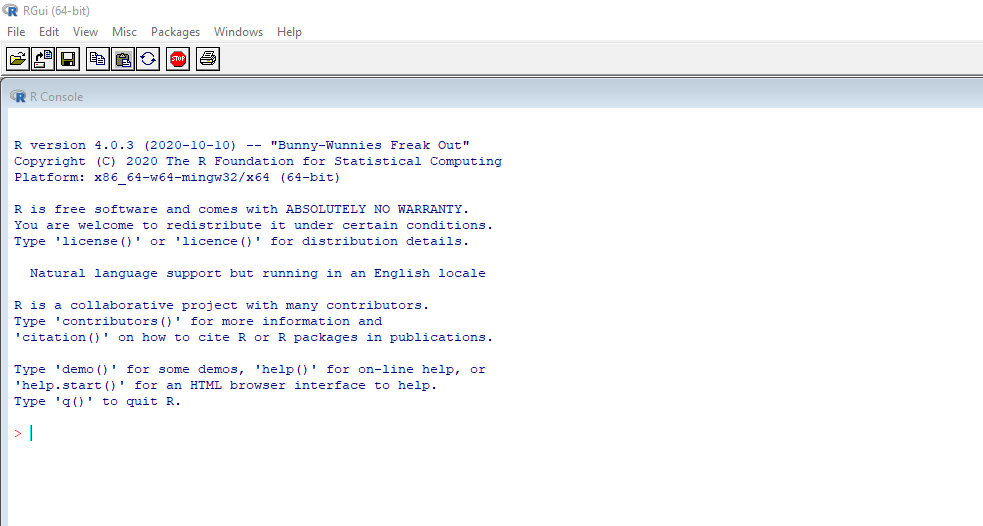
\includegraphics[width=0.85\linewidth]{images/r-console} 

}

\caption{La console di R, solo per veri intenditori}\label{fig:r-console}
\end{figure}

\hypertarget{script-il-tuo-blocco-appunti}{%
\subsection{Script: Il tuo Blocco Appunti}\label{script-il-tuo-blocco-appunti}}

\hypertarget{console-il-cuore-di-r}{%
\subsection{Console: Il Cuore di R}\label{console-il-cuore-di-r}}

\hypertarget{environment-e-history-lambiente-di-lavoro}{%
\subsection{Environment e History: L'Ambiente di Lavoro}\label{environment-e-history-lambiente-di-lavoro}}

\hypertarget{file-plots-package-help-system-management}{%
\subsection{File, Plots, Package, Help: System Management}\label{file-plots-package-help-system-management}}

\hypertarget{approfondimento-personalizzazione-layout-e-theme}{%
\subsubsection{approfondimento personalizzazione layout e theme}\label{approfondimento-personalizzazione-layout-e-theme}}

\hypertarget{primi-comandi}{%
\section{Primi Comandi}\label{primi-comandi}}

\hypertarget{operatori-matematici}{%
\subsection{Operatori Matematici}\label{operatori-matematici}}

\hypertarget{operatori-logici}{%
\subsection{Operatori Logici}\label{operatori-logici}}

\hypertarget{approfondimento-operatore-in}{%
\subsubsection{\texorpdfstring{approfondimento operatore \texttt{\%in\%}}{approfondimento operatore \%in\%}}\label{approfondimento-operatore-in}}

\hypertarget{creazione-di-variabili}{%
\section{Creazione di Variabili}\label{creazione-di-variabili}}

concetto di variabile e assegnare i valori

\hypertarget{approfondimento-diversi-modi-di-assegnare-un-valore---assign}{%
\subsubsection{\texorpdfstring{approfondimento diversi modi di ``assegnare un valore'' (\texttt{\textless{}-}, \texttt{=}, \texttt{assign()})}{approfondimento diversi modi di ``assegnare un valore'' (\textless-, =, assign())}}\label{approfondimento-diversi-modi-di-assegnare-un-valore---assign}}

\hypertarget{utilizzo-di-funzioni}{%
\section{Utilizzo di funzioni}\label{utilizzo-di-funzioni}}

\hypertarget{section}{%
\subsection{}\label{section}}

\hypertarget{working-session}{%
\chapter{Sessione di Lavoro}\label{working-session}}

Working in progress.

\hypertarget{infobox}{%
\section{Infobox}\label{infobox}}

Illustrations included in \texttt{images/} are retrieved from \href{https://rstudio4edu.github.io/rstudio4edu-book/}{rstudio4edu-book} under \href{https://creativecommons.org/licenses/by-nc/2.0/}{CC-BY-NC}. Remember to include an \emph{Attributions} section in the book and repository's README file.

\begin{tip}[My title]

Lorem ipsum dolor sit amet consectetur adipisicing elit. Maxime mollitia,
molestiae quas vel sint commodi repudiandae consequuntur voluptatum laborum
numquam blanditiis harum quisquam eius sed odit fugiat iusto fuga praesentium
optio, eaque rerum!

\end{tip}

\begin{warning}[My title]

Lorem ipsum dolor sit amet consectetur adipisicing elit. Maxime mollitia,
molestiae quas vel sint commodi repudiandae consequuntur voluptatum laborum
numquam blanditiis harum quisquam eius sed odit fugiat iusto fuga praesentium
optio, eaque rerum!

\end{warning}

\begin{deffun}[My title]

Lorem ipsum dolor sit amet consectetur adipisicing elit. Maxime mollitia,
molestiae quas vel sint commodi repudiandae consequuntur voluptatum laborum
numquam blanditiis harum quisquam eius sed odit fugiat iusto fuga praesentium
optio, eaque rerum!

\end{deffun}

\begin{design}[My title]

Lorem ipsum dolor sit amet consectetur adipisicing elit. Maxime mollitia,
molestiae quas vel sint commodi repudiandae consequuntur voluptatum laborum
numquam blanditiis harum quisquam eius sed odit fugiat iusto fuga praesentium
optio, eaque rerum!

\end{design}

\begin{trick}[My title]

Lorem ipsum dolor sit amet consectetur adipisicing elit. Maxime mollitia,
molestiae quas vel sint commodi repudiandae consequuntur voluptatum laborum
numquam blanditiis harum quisquam eius sed odit fugiat iusto fuga praesentium
optio, eaque rerum!

\end{trick}

\hypertarget{part-struttura-dati}{%
\part*{Struttura Dati}\label{part-struttura-dati}}
\addcontentsline{toc}{part}{Struttura Dati}

\hypertarget{introduzione}{%
\chapter*{Introduzione}\label{introduzione}}
\addcontentsline{toc}{chapter}{Introduzione}

Working in progress.

\hypertarget{vector}{%
\chapter{Vettori}\label{vector}}

Working in progress.

\hypertarget{matrix}{%
\chapter{Matrici}\label{matrix}}

Working in progress.

\hypertarget{dataframe}{%
\chapter{Dataframe}\label{dataframe}}

Working in progress.

\hypertarget{list}{%
\chapter{Liste}\label{list}}

Working in progress.

\hypertarget{part-algoritmi}{%
\part*{Algoritmi}\label{part-algoritmi}}
\addcontentsline{toc}{part}{Algoritmi}

\hypertarget{introduzione-1}{%
\chapter*{Introduzione}\label{introduzione-1}}
\addcontentsline{toc}{chapter}{Introduzione}

Working in progress.

\hypertarget{functions}{%
\chapter{Definizione di Funzioni}\label{functions}}

Working in progress.

\hypertarget{coditionals}{%
\chapter{Programmazione Condizionale}\label{coditionals}}

Working in progress.

\hypertarget{loop}{%
\chapter{Attenti al loop}\label{loop}}

Working in progress.

\hypertarget{part-case-study}{%
\part*{Case study}\label{part-case-study}}
\addcontentsline{toc}{part}{Case study}

\hypertarget{introduzione-2}{%
\chapter*{Introduzione}\label{introduzione-2}}
\addcontentsline{toc}{chapter}{Introduzione}

Working in progress.

\hypertarget{attachment}{%
\chapter{Caso Studio I: Attaccamento}\label{attachment}}

Working in progress.

  \bibliography{book.bib,packages.bib}

\end{document}
